\documentclass[twoside]{book}

% Packages required by doxygen
\usepackage{fixltx2e}
\usepackage{calc}
\usepackage{doxygen}
\usepackage{graphicx}
\usepackage[utf8]{inputenc}
\usepackage{makeidx}
\usepackage{multicol}
\usepackage{multirow}
\PassOptionsToPackage{warn}{textcomp}
\usepackage{textcomp}
\usepackage[nointegrals]{wasysym}
\usepackage[table]{xcolor}

% Font selection
\usepackage[T1]{fontenc}
\usepackage{mathptmx}
\usepackage[scaled=.90]{helvet}
\usepackage{courier}
\usepackage{amssymb}
\usepackage{sectsty}
\renewcommand{\familydefault}{\sfdefault}
\allsectionsfont{%
  \fontseries{bc}\selectfont%
  \color{darkgray}%
}
\renewcommand{\DoxyLabelFont}{%
  \fontseries{bc}\selectfont%
  \color{darkgray}%
}
\newcommand{\+}{\discretionary{\mbox{\scriptsize$\hookleftarrow$}}{}{}}

% Page & text layout
\usepackage{geometry}
\geometry{%
  a4paper,%
  top=2.5cm,%
  bottom=2.5cm,%
  left=2.5cm,%
  right=2.5cm%
}
\tolerance=750
\hfuzz=15pt
\hbadness=750
\setlength{\emergencystretch}{15pt}
\setlength{\parindent}{0cm}
\setlength{\parskip}{0.2cm}
\makeatletter
\renewcommand{\paragraph}{%
  \@startsection{paragraph}{4}{0ex}{-1.0ex}{1.0ex}{%
    \normalfont\normalsize\bfseries\SS@parafont%
  }%
}
\renewcommand{\subparagraph}{%
  \@startsection{subparagraph}{5}{0ex}{-1.0ex}{1.0ex}{%
    \normalfont\normalsize\bfseries\SS@subparafont%
  }%
}
\makeatother

% Headers & footers
\usepackage{fancyhdr}
\pagestyle{fancyplain}
\fancyhead[LE]{\fancyplain{}{\bfseries\thepage}}
\fancyhead[CE]{\fancyplain{}{}}
\fancyhead[RE]{\fancyplain{}{\bfseries\leftmark}}
\fancyhead[LO]{\fancyplain{}{\bfseries\rightmark}}
\fancyhead[CO]{\fancyplain{}{}}
\fancyhead[RO]{\fancyplain{}{\bfseries\thepage}}
\fancyfoot[LE]{\fancyplain{}{}}
\fancyfoot[CE]{\fancyplain{}{}}
\fancyfoot[RE]{\fancyplain{}{\bfseries\scriptsize Generated on Wed Oct 29 2014 12\+:11\+:33 for Open\+G\+L Toolbox by Doxygen }}
\fancyfoot[LO]{\fancyplain{}{\bfseries\scriptsize Generated on Wed Oct 29 2014 12\+:11\+:33 for Open\+G\+L Toolbox by Doxygen }}
\fancyfoot[CO]{\fancyplain{}{}}
\fancyfoot[RO]{\fancyplain{}{}}
\renewcommand{\footrulewidth}{0.4pt}
\renewcommand{\chaptermark}[1]{%
  \markboth{#1}{}%
}
\renewcommand{\sectionmark}[1]{%
  \markright{\thesection\ #1}%
}

% Indices & bibliography
\usepackage{natbib}
\usepackage[titles]{tocloft}
\setcounter{tocdepth}{3}
\setcounter{secnumdepth}{5}
\makeindex

% Hyperlinks (required, but should be loaded last)
\usepackage{ifpdf}
\ifpdf
  \usepackage[pdftex,pagebackref=true]{hyperref}
\else
  \usepackage[ps2pdf,pagebackref=true]{hyperref}
\fi
\hypersetup{%
  colorlinks=true,%
  linkcolor=blue,%
  citecolor=blue,%
  unicode%
}

% Custom commands
\newcommand{\clearemptydoublepage}{%
  \newpage{\pagestyle{empty}\cleardoublepage}%
}


%===== C O N T E N T S =====

\begin{document}

% Titlepage & ToC
\hypersetup{pageanchor=false,
             bookmarks=true,
             bookmarksnumbered=true,
             pdfencoding=unicode
            }
\pagenumbering{roman}
\begin{titlepage}
\vspace*{7cm}
\begin{center}%
{\Large Open\+G\+L Toolbox \\[1ex]\large 0.\+1 }\\
\vspace*{1cm}
{\large Generated by Doxygen 1.8.8}\\
\vspace*{0.5cm}
{\small Wed Oct 29 2014 12:11:33}\\
\end{center}
\end{titlepage}
\clearemptydoublepage
\tableofcontents
\clearemptydoublepage
\pagenumbering{arabic}
\hypersetup{pageanchor=true}

%--- Begin generated contents ---
\chapter{Todo List}
\label{todo}
\hypertarget{todo}{}

\begin{DoxyRefList}
\item[\label{todo__todo000001}%
\hypertarget{todo__todo000001}{}%
Class \hyperlink{class_cubic_spline}{Cubic\+Spline$<$ T, R $>$} ]Easier point insertion ? Auto sorting if time is specified ? 

Comment the whole thing
\end{DoxyRefList}
\chapter{Hierarchical Index}
\section{Class Hierarchy}
This inheritance list is sorted roughly, but not completely, alphabetically\+:\begin{DoxyCompactList}
\item \contentsline{section}{Camera}{\pageref{class_camera}}{}
\item \contentsline{section}{chunk}{\pageref{structchunk}}{}
\item \contentsline{section}{Cubic\+Spline$<$ T, R $>$\+:\+:Control\+Point}{\pageref{class_cubic_spline_1_1_control_point}}{}
\item \contentsline{section}{Cubic\+Spline$<$ T, R $>$}{\pageref{class_cubic_spline}}{}
\item \contentsline{section}{Curve$<$ T, R $>$}{\pageref{class_curve}}{}
\begin{DoxyCompactList}
\item \contentsline{section}{Bezier$<$ T, R $>$}{\pageref{class_bezier}}{}
\end{DoxyCompactList}
\item \contentsline{section}{Framebuffer$<$ Cube\+Map $>$}{\pageref{class_framebuffer_3_01_cube_map_01_4}}{}
\item \contentsline{section}{Frustum}{\pageref{class_frustum}}{}
\item \contentsline{section}{Generic\+Uniform}{\pageref{class_generic_uniform}}{}
\begin{DoxyCompactList}
\item \contentsline{section}{Uniform$<$ T $>$}{\pageref{class_uniform}}{}
\item \contentsline{section}{Uniform$<$ Texture $>$}{\pageref{class_uniform_3_01_texture_01_4}}{}
\end{DoxyCompactList}
\item \contentsline{section}{huffman}{\pageref{structhuffman}}{}
\item \contentsline{section}{jpeg}{\pageref{structjpeg}}{}
\item \contentsline{section}{Light}{\pageref{class_light}}{}
\item \contentsline{section}{Material}{\pageref{class_material}}{}
\item Open\+G\+L\+Object\begin{DoxyCompactList}
\item \contentsline{section}{Framebuffer$<$ Tex\+Type $>$}{\pageref{class_framebuffer}}{}
\item \contentsline{section}{Texture}{\pageref{class_texture}}{}
\begin{DoxyCompactList}
\item \contentsline{section}{Cube\+Map}{\pageref{class_cube_map}}{}
\item \contentsline{section}{Texture2\+D}{\pageref{class_texture2_d}}{}
\end{DoxyCompactList}
\end{DoxyCompactList}
\item \contentsline{section}{pic\+\_\+packet\+\_\+t}{\pageref{structpic__packet__t}}{}
\item \contentsline{section}{Plane}{\pageref{class_plane}}{}
\item \contentsline{section}{png}{\pageref{structpng}}{}
\item \contentsline{section}{Program}{\pageref{class_program}}{}
\item \contentsline{section}{Shader}{\pageref{class_shader}}{}
\begin{DoxyCompactList}
\item \contentsline{section}{Compute\+Shader}{\pageref{class_compute_shader}}{}
\item \contentsline{section}{Fragment\+Shader}{\pageref{class_fragment_shader}}{}
\item \contentsline{section}{Geometry\+Shader}{\pageref{class_geometry_shader}}{}
\item \contentsline{section}{Vertex\+Shader}{\pageref{class_vertex_shader}}{}
\end{DoxyCompactList}
\item \contentsline{section}{Singleton$<$ C $>$}{\pageref{class_singleton}}{}
\item \contentsline{section}{Singleton$<$ Resources\+Manager $>$}{\pageref{class_singleton}}{}
\begin{DoxyCompactList}
\item \contentsline{section}{Resources\+Manager}{\pageref{class_resources_manager}}{}
\end{DoxyCompactList}
\item \contentsline{section}{Singleton$<$ Time\+Manager $>$}{\pageref{class_singleton}}{}
\begin{DoxyCompactList}
\item \contentsline{section}{Time\+Manager}{\pageref{class_time_manager}}{}
\end{DoxyCompactList}
\item \contentsline{section}{Skybox}{\pageref{class_skybox}}{}
\item \contentsline{section}{stbi}{\pageref{structstbi}}{}
\item \contentsline{section}{stbi\+\_\+gif\+\_\+lzw\+\_\+struct}{\pageref{structstbi__gif__lzw__struct}}{}
\item \contentsline{section}{stbi\+\_\+gif\+\_\+struct}{\pageref{structstbi__gif__struct}}{}
\item \contentsline{section}{stbi\+\_\+io\+\_\+callbacks}{\pageref{structstbi__io__callbacks}}{}
\item \contentsline{section}{stbi\+\_\+resample}{\pageref{structstbi__resample}}{}
\item \contentsline{section}{Timer}{\pageref{class_timer}}{}
\item \contentsline{section}{Material\+:\+:Uniform$<$ T $>$}{\pageref{class_material_1_1_uniform}}{}
\item \contentsline{section}{zbuf}{\pageref{structzbuf}}{}
\item \contentsline{section}{zhuffman}{\pageref{structzhuffman}}{}
\end{DoxyCompactList}

\chapter{Class Index}
\section{Class List}
Here are the classes, structs, unions and interfaces with brief descriptions\+:\begin{DoxyCompactList}
\item\contentsline{section}{\hyperlink{class_bezier}{Bezier$<$ T, R $>$} }{\pageref{class_bezier}}{}
\item\contentsline{section}{\hyperlink{class_camera}{Camera} }{\pageref{class_camera}}{}
\item\contentsline{section}{\hyperlink{structchunk}{chunk} }{\pageref{structchunk}}{}
\item\contentsline{section}{\hyperlink{class_compute_shader}{Compute\+Shader} }{\pageref{class_compute_shader}}{}
\item\contentsline{section}{\hyperlink{class_cubic_spline_1_1_control_point}{Cubic\+Spline$<$ T, R $>$\+::\+Control\+Point} }{\pageref{class_cubic_spline_1_1_control_point}}{}
\item\contentsline{section}{\hyperlink{class_cube_map}{Cube\+Map} }{\pageref{class_cube_map}}{}
\item\contentsline{section}{\hyperlink{class_cubic_spline}{Cubic\+Spline$<$ T, R $>$} }{\pageref{class_cubic_spline}}{}
\item\contentsline{section}{\hyperlink{class_curve}{Curve$<$ T, R $>$} }{\pageref{class_curve}}{}
\item\contentsline{section}{\hyperlink{class_fragment_shader}{Fragment\+Shader} }{\pageref{class_fragment_shader}}{}
\item\contentsline{section}{\hyperlink{class_framebuffer}{Framebuffer$<$ Tex\+Type $>$} }{\pageref{class_framebuffer}}{}
\item\contentsline{section}{\hyperlink{class_framebuffer_3_01_cube_map_01_4}{Framebuffer$<$ Cube\+Map $>$} }{\pageref{class_framebuffer_3_01_cube_map_01_4}}{}
\item\contentsline{section}{\hyperlink{class_frustum}{Frustum} }{\pageref{class_frustum}}{}
\item\contentsline{section}{\hyperlink{class_generic_uniform}{Generic\+Uniform} }{\pageref{class_generic_uniform}}{}
\item\contentsline{section}{\hyperlink{class_geometry_shader}{Geometry\+Shader} }{\pageref{class_geometry_shader}}{}
\item\contentsline{section}{\hyperlink{structhuffman}{huffman} }{\pageref{structhuffman}}{}
\item\contentsline{section}{\hyperlink{structjpeg}{jpeg} }{\pageref{structjpeg}}{}
\item\contentsline{section}{\hyperlink{class_light}{Light} }{\pageref{class_light}}{}
\item\contentsline{section}{\hyperlink{class_material}{Material} }{\pageref{class_material}}{}
\item\contentsline{section}{\hyperlink{structpic__packet__t}{pic\+\_\+packet\+\_\+t} }{\pageref{structpic__packet__t}}{}
\item\contentsline{section}{\hyperlink{class_plane}{Plane} }{\pageref{class_plane}}{}
\item\contentsline{section}{\hyperlink{structpng}{png} }{\pageref{structpng}}{}
\item\contentsline{section}{\hyperlink{class_program}{Program} }{\pageref{class_program}}{}
\item\contentsline{section}{\hyperlink{class_resources_manager}{Resources\+Manager} }{\pageref{class_resources_manager}}{}
\item\contentsline{section}{\hyperlink{class_shader}{Shader} }{\pageref{class_shader}}{}
\item\contentsline{section}{\hyperlink{class_singleton}{Singleton$<$ C $>$} \\*Abstract class for singleton pattern }{\pageref{class_singleton}}{}
\item\contentsline{section}{\hyperlink{class_skybox}{Skybox} }{\pageref{class_skybox}}{}
\item\contentsline{section}{\hyperlink{structstbi}{stbi} }{\pageref{structstbi}}{}
\item\contentsline{section}{\hyperlink{structstbi__gif__lzw__struct}{stbi\+\_\+gif\+\_\+lzw\+\_\+struct} }{\pageref{structstbi__gif__lzw__struct}}{}
\item\contentsline{section}{\hyperlink{structstbi__gif__struct}{stbi\+\_\+gif\+\_\+struct} }{\pageref{structstbi__gif__struct}}{}
\item\contentsline{section}{\hyperlink{structstbi__io__callbacks}{stbi\+\_\+io\+\_\+callbacks} }{\pageref{structstbi__io__callbacks}}{}
\item\contentsline{section}{\hyperlink{structstbi__resample}{stbi\+\_\+resample} }{\pageref{structstbi__resample}}{}
\item\contentsline{section}{\hyperlink{class_texture}{Texture} }{\pageref{class_texture}}{}
\item\contentsline{section}{\hyperlink{class_texture2_d}{Texture2\+D} }{\pageref{class_texture2_d}}{}
\item\contentsline{section}{\hyperlink{class_time_manager}{Time\+Manager} }{\pageref{class_time_manager}}{}
\item\contentsline{section}{\hyperlink{class_timer}{Timer} }{\pageref{class_timer}}{}
\item\contentsline{section}{\hyperlink{class_uniform}{Uniform$<$ T $>$} }{\pageref{class_uniform}}{}
\item\contentsline{section}{\hyperlink{class_material_1_1_uniform}{Material\+::\+Uniform$<$ T $>$} }{\pageref{class_material_1_1_uniform}}{}
\item\contentsline{section}{\hyperlink{class_uniform_3_01_texture_01_4}{Uniform$<$ Texture $>$} }{\pageref{class_uniform_3_01_texture_01_4}}{}
\item\contentsline{section}{\hyperlink{class_vertex_shader}{Vertex\+Shader} }{\pageref{class_vertex_shader}}{}
\item\contentsline{section}{\hyperlink{structzbuf}{zbuf} }{\pageref{structzbuf}}{}
\item\contentsline{section}{\hyperlink{structzhuffman}{zhuffman} }{\pageref{structzhuffman}}{}
\end{DoxyCompactList}

\chapter{Class Documentation}
\hypertarget{class_bezier}{\section{Bezier$<$ T, R $>$ Class Template Reference}
\label{class_bezier}\index{Bezier$<$ T, R $>$@{Bezier$<$ T, R $>$}}
}
Inheritance diagram for Bezier$<$ T, R $>$\+:\begin{figure}[H]
\begin{center}
\leavevmode
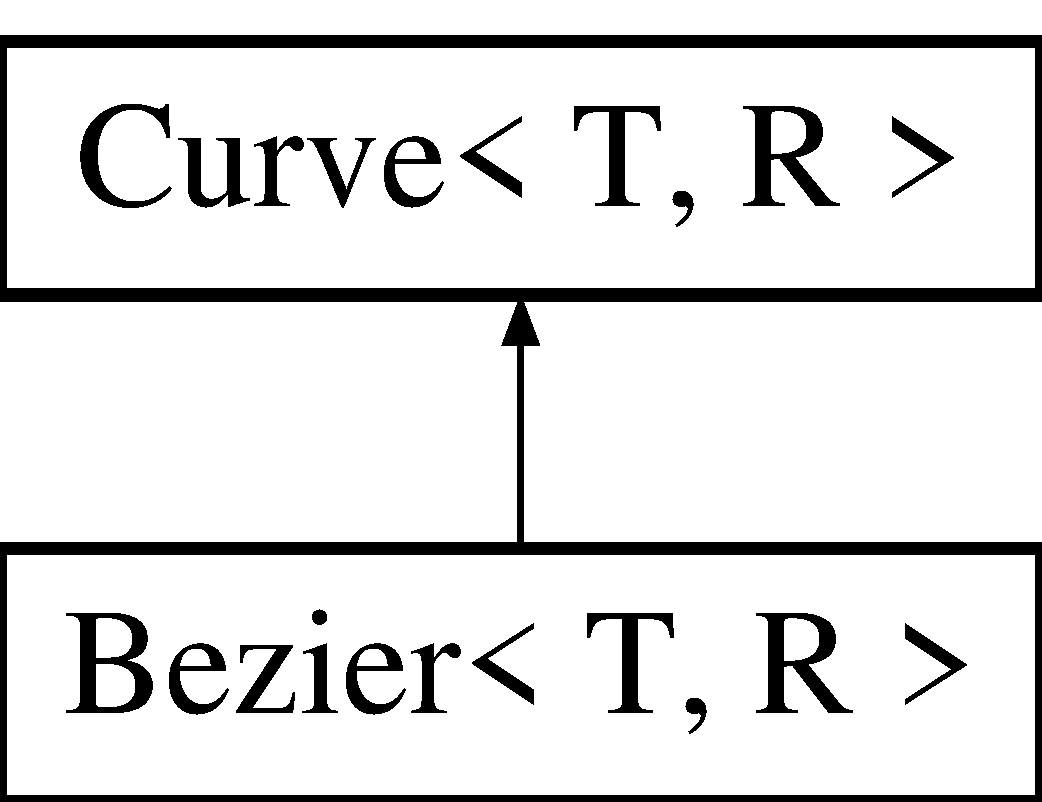
\includegraphics[height=2.000000cm]{class_bezier}
\end{center}
\end{figure}
\subsection*{Public Member Functions}
\begin{DoxyCompactItemize}
\item 
\hypertarget{class_bezier_a7708810890b783088efcc9110ca130bc}{{\bfseries Bezier} (const \hyperlink{class_curve}{Curve}$<$ T, R $>$ \&C, size\+\_\+t precision=100)}\label{class_bezier_a7708810890b783088efcc9110ca130bc}

\item 
\hypertarget{class_bezier_a0886f7c2af8fe37bbd8b10b3ea208ef4}{{\bfseries Bezier} (const std\+::initializer\+\_\+list$<$ T $>$ \&L, size\+\_\+t precision=100)}\label{class_bezier_a0886f7c2af8fe37bbd8b10b3ea208ef4}

\item 
\hypertarget{class_bezier_a48c90931037d5f17ea0e17380ebbd194}{{\footnotesize template$<$class Iterator $>$ }\\{\bfseries Bezier} (Iterator Begin, Iterator End, size\+\_\+t precision=100)}\label{class_bezier_a48c90931037d5f17ea0e17380ebbd194}

\item 
\hypertarget{class_bezier_a61a72b2602f471e3b60196cc2f685efb}{void {\bfseries compute} (size\+\_\+t precision=100)}\label{class_bezier_a61a72b2602f471e3b60196cc2f685efb}

\item 
\hypertarget{class_bezier_a5e87845baa70d59e2c5a14c2155b00ee}{size\+\_\+t {\bfseries get\+Control\+Point\+Count} ()}\label{class_bezier_a5e87845baa70d59e2c5a14c2155b00ee}

\item 
\hypertarget{class_bezier_ab27b6b7a62d2f1765fb4dc89337baf8d}{\hyperlink{class_bezier}{Bezier}$<$ T, R $>$ \& {\bfseries operator+=} (const T \&V)}\label{class_bezier_ab27b6b7a62d2f1765fb4dc89337baf8d}

\item 
\hypertarget{class_bezier_a19985473de96c4718860bd2568084b53}{void {\bfseries reset} ()}\label{class_bezier_a19985473de96c4718860bd2568084b53}

\end{DoxyCompactItemize}
\subsection*{Additional Inherited Members}


The documentation for this class was generated from the following file\+:\begin{DoxyCompactItemize}
\item 
src/Bezier.\+hpp\end{DoxyCompactItemize}

\hypertarget{class_camera}{\section{Camera Class Reference}
\label{class_camera}\index{Camera@{Camera}}
}
\subsection*{Public Member Functions}
\begin{DoxyCompactItemize}
\item 
\hypertarget{class_camera_aa0da8772ff7e4c9d4a12b9b5613ee131}{{\bfseries Camera} (glm\+::vec3 position=Base\+Position, glm\+::vec3 direction=Base\+Direction, glm\+::vec3 up=Base\+Up, float speed=Base\+Speed, float sensitivity=Base\+Sensitivity)}\label{class_camera_aa0da8772ff7e4c9d4a12b9b5613ee131}

\item 
\hypertarget{class_camera_aa404ef2bd024a357ca003cff9c78d32d}{void {\bfseries strafe\+Right} (float dt=1.f)}\label{class_camera_aa404ef2bd024a357ca003cff9c78d32d}

\item 
\hypertarget{class_camera_aa4670614ca81adb41cd298d0ea54c2a4}{void {\bfseries strafe\+Left} (float dt=1.f)}\label{class_camera_aa4670614ca81adb41cd298d0ea54c2a4}

\item 
\hypertarget{class_camera_a8b313687db6609c0ca037e051de4b42e}{void {\bfseries move\+Forward} (float dt=1.f)}\label{class_camera_a8b313687db6609c0ca037e051de4b42e}

\item 
\hypertarget{class_camera_aa2a60abcd657abc23dcf7e336a8dbf44}{void {\bfseries move\+Backward} (float dt=1.f)}\label{class_camera_aa2a60abcd657abc23dcf7e336a8dbf44}

\item 
\hypertarget{class_camera_a78468098bdb8a2bdf3217510be56e2f6}{void {\bfseries move\+Up} (float dt=1.f)}\label{class_camera_a78468098bdb8a2bdf3217510be56e2f6}

\item 
\hypertarget{class_camera_ac42144cc0087d84ef87a0c51a08474ae}{void {\bfseries move\+Down} (float dt=1.f)}\label{class_camera_ac42144cc0087d84ef87a0c51a08474ae}

\item 
\hypertarget{class_camera_a8724a80dee180185e236634d72040e04}{void {\bfseries look} (glm\+::vec2 v)}\label{class_camera_a8724a80dee180185e236634d72040e04}

\item 
\hypertarget{class_camera_a84fd8b7dc4e2f00fb0bb43c462bfc71d}{void {\bfseries update\+View} ()}\label{class_camera_a84fd8b7dc4e2f00fb0bb43c462bfc71d}

\item 
\hypertarget{class_camera_a02be8aa0dbef77e02dddc715a726fb67}{void {\bfseries reset} ()}\label{class_camera_a02be8aa0dbef77e02dddc715a726fb67}

\item 
\hypertarget{class_camera_afa9614890e5e4d2613a940381a5d1863}{const glm\+::mat4 \& {\bfseries get\+Matrix} () const }\label{class_camera_afa9614890e5e4d2613a940381a5d1863}

\item 
\hypertarget{class_camera_ab7ebcdd5020d8057f1df3bdb33bac456}{void {\bfseries set\+Position} (const glm\+::vec3 \&pos)}\label{class_camera_ab7ebcdd5020d8057f1df3bdb33bac456}

\item 
\hypertarget{class_camera_ad4740221f8d5cb38d7723dbbf2493f1c}{void {\bfseries set\+Direction} (const glm\+::vec3 \&dir)}\label{class_camera_ad4740221f8d5cb38d7723dbbf2493f1c}

\item 
\hypertarget{class_camera_a1a371757084da11766d4efec19d5092f}{void {\bfseries look\+At} (const glm\+::vec3 \&at)}\label{class_camera_a1a371757084da11766d4efec19d5092f}

\item 
\hypertarget{class_camera_ae206a19d576b3292b63d47581a7aa955}{glm\+::vec3 \& {\bfseries get\+Position} ()}\label{class_camera_ae206a19d576b3292b63d47581a7aa955}

\item 
\hypertarget{class_camera_ac3f20f73b8e37f445da786bfe9e33690}{const glm\+::vec3 \& {\bfseries get\+Position} () const }\label{class_camera_ac3f20f73b8e37f445da786bfe9e33690}

\item 
\hypertarget{class_camera_a098942f443a5a7edfe21f4ccd680efc8}{const glm\+::vec3 \& {\bfseries get\+Direction} () const }\label{class_camera_a098942f443a5a7edfe21f4ccd680efc8}

\item 
\hypertarget{class_camera_a8369f3a557efe04e62e8abe81aa4cf77}{const glm\+::vec3 \& {\bfseries get\+Up} () const }\label{class_camera_a8369f3a557efe04e62e8abe81aa4cf77}

\item 
\hypertarget{class_camera_a73962ae24996182b70373639ee80e653}{float \& {\bfseries speed} ()}\label{class_camera_a73962ae24996182b70373639ee80e653}

\item 
\hypertarget{class_camera_a4c6077aea1f998143942d0e1b28d1ddb}{float \& {\bfseries sensitivity} ()}\label{class_camera_a4c6077aea1f998143942d0e1b28d1ddb}

\end{DoxyCompactItemize}


The documentation for this class was generated from the following files\+:\begin{DoxyCompactItemize}
\item 
src/\+Graphics/Camera.\+hpp\item 
src/\+Graphics/Camera.\+cpp\end{DoxyCompactItemize}

\hypertarget{structchunk}{\section{chunk Struct Reference}
\label{structchunk}\index{chunk@{chunk}}
}
\subsection*{Public Attributes}
\begin{DoxyCompactItemize}
\item 
\hypertarget{structchunk_a0b5cc0c5a9b91945c42373db2a499fb1}{uint32 {\bfseries length}}\label{structchunk_a0b5cc0c5a9b91945c42373db2a499fb1}

\item 
\hypertarget{structchunk_a05d5489f3807bc7ba149c1904241d087}{uint32 {\bfseries type}}\label{structchunk_a05d5489f3807bc7ba149c1904241d087}

\end{DoxyCompactItemize}


The documentation for this struct was generated from the following file\+:\begin{DoxyCompactItemize}
\item 
src/\+Graphics/stb\+\_\+image.\+cpp\end{DoxyCompactItemize}

\hypertarget{class_compute_shader}{\section{Compute\+Shader Class Reference}
\label{class_compute_shader}\index{Compute\+Shader@{Compute\+Shader}}
}
Inheritance diagram for Compute\+Shader\+:\begin{figure}[H]
\begin{center}
\leavevmode
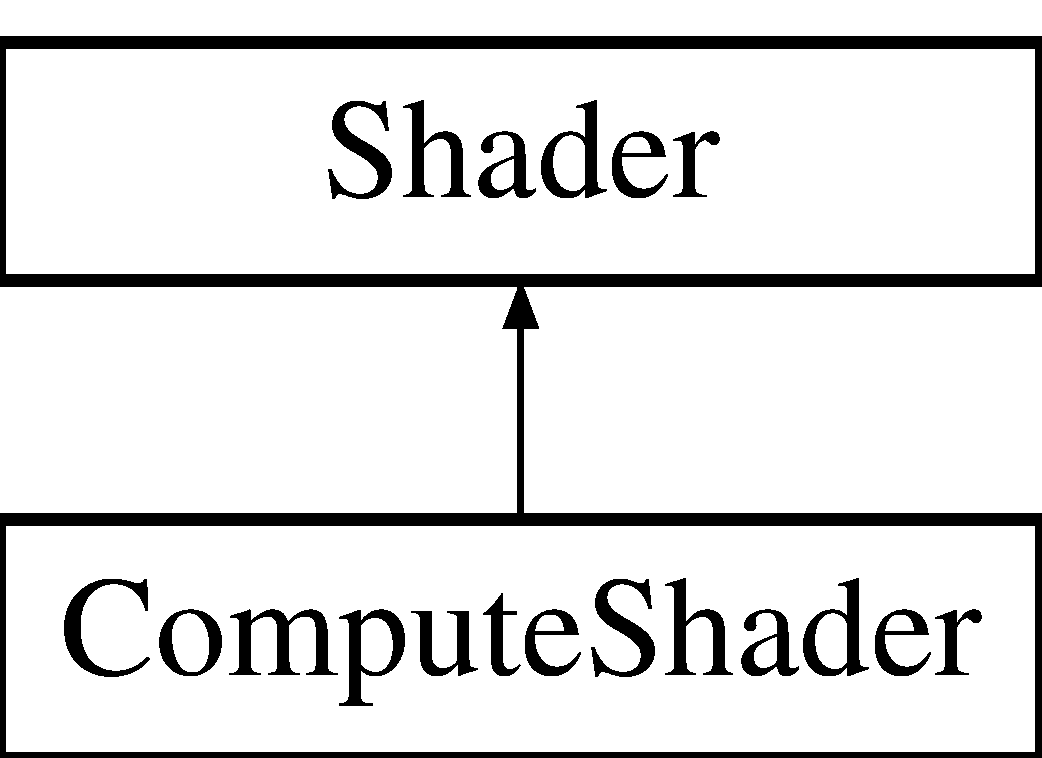
\includegraphics[height=2.000000cm]{class_compute_shader}
\end{center}
\end{figure}
\subsection*{Public Member Functions}
\begin{DoxyCompactItemize}
\item 
\hypertarget{class_compute_shader_a818f0e0836fa20a0f929c311a69bbb4b}{{\bfseries Compute\+Shader} (bool standalone=true)}\label{class_compute_shader_a818f0e0836fa20a0f929c311a69bbb4b}

\item 
\hypertarget{class_compute_shader_ac86652bbfdac9b93727da048e1b5a8aa}{void {\bfseries compile} ()}\label{class_compute_shader_ac86652bbfdac9b93727da048e1b5a8aa}

\item 
\hypertarget{class_compute_shader_a252c0422abdc92a1492dcd0255450fa9}{void {\bfseries use} ()}\label{class_compute_shader_a252c0422abdc92a1492dcd0255450fa9}

\item 
\hypertarget{class_compute_shader_a18cf7de584c2b0ba519f71adb9d232c1}{void {\bfseries compute} (G\+Lint x, G\+Lint y=1, G\+Lint z=1)}\label{class_compute_shader_a18cf7de584c2b0ba519f71adb9d232c1}

\item 
\hypertarget{class_compute_shader_a092e90d32702a438956480e5f4ff3f08}{G\+Lint {\bfseries get\+Program\+I\+D} () const }\label{class_compute_shader_a092e90d32702a438956480e5f4ff3f08}

\end{DoxyCompactItemize}
\subsection*{Static Public Member Functions}
\begin{DoxyCompactItemize}
\item 
\hypertarget{class_compute_shader_a01fe703554fc9844e5f16c8860c2e44b}{static void {\bfseries memory\+Barrier} (G\+Lbitfield B\+F=G\+L\+\_\+\+A\+L\+L\+\_\+\+B\+A\+R\+R\+I\+E\+R\+\_\+\+B\+I\+T\+S)}\label{class_compute_shader_a01fe703554fc9844e5f16c8860c2e44b}

\item 
\hypertarget{class_compute_shader_ade055daefa7afb6c0ef8ec7ff27828ff}{static void {\bfseries dispatch\+Compute} (G\+Lint x, G\+Lint y=1, G\+Lint z=1)}\label{class_compute_shader_ade055daefa7afb6c0ef8ec7ff27828ff}

\end{DoxyCompactItemize}
\subsection*{Friends}
\begin{DoxyCompactItemize}
\item 
\hypertarget{class_compute_shader_a0432bf4ab621f4098afac914ccb5371e}{class {\bfseries Program}}\label{class_compute_shader_a0432bf4ab621f4098afac914ccb5371e}

\end{DoxyCompactItemize}
\subsection*{Additional Inherited Members}


The documentation for this class was generated from the following files\+:\begin{DoxyCompactItemize}
\item 
src/\+Graphics/\+Shader\+Program/Compute\+Shader.\+hpp\item 
src/\+Graphics/\+Shader\+Program/Compute\+Shader.\+cpp\end{DoxyCompactItemize}

\hypertarget{class_cubic_spline_1_1_control_point}{\section{Cubic\+Spline$<$ T, R $>$\+:\+:Control\+Point Class Reference}
\label{class_cubic_spline_1_1_control_point}\index{Cubic\+Spline$<$ T, R $>$\+::\+Control\+Point@{Cubic\+Spline$<$ T, R $>$\+::\+Control\+Point}}
}


{\ttfamily \#include $<$Cubic\+Spline.\+hpp$>$}

\subsection*{Public Member Functions}
\begin{DoxyCompactItemize}
\item 
\hypertarget{class_cubic_spline_1_1_control_point_af599da00be5d4c064ff8f014147aa97e}{{\bfseries Control\+Point} (const \hyperlink{class_cubic_spline_1_1_control_point}{Control\+Point} \&)=default}\label{class_cubic_spline_1_1_control_point_af599da00be5d4c064ff8f014147aa97e}

\item 
\hypertarget{class_cubic_spline_1_1_control_point_a60e070a59f5e4e952dfde49e273f6c29}{{\bfseries Control\+Point} (\hyperlink{class_cubic_spline_1_1_control_point}{Control\+Point} \&\&)=default}\label{class_cubic_spline_1_1_control_point_a60e070a59f5e4e952dfde49e273f6c29}

\item 
\hypertarget{class_cubic_spline_1_1_control_point_abe4fb6190bbabd312f9ed5148edd1b79}{{\bfseries Control\+Point} (T position, T speed=T(), R time=R())}\label{class_cubic_spline_1_1_control_point_abe4fb6190bbabd312f9ed5148edd1b79}

\item 
\hypertarget{class_cubic_spline_1_1_control_point_a7b40d5fd4c424527bc3f14b684d2220e}{bool \hyperlink{class_cubic_spline_1_1_control_point_a7b40d5fd4c424527bc3f14b684d2220e}{is\+Dirty} () const }\label{class_cubic_spline_1_1_control_point_a7b40d5fd4c424527bc3f14b684d2220e}

\begin{DoxyCompactList}\small\item\em Should not be used outside of \hyperlink{class_cubic_spline}{Cubic\+Spline}. \end{DoxyCompactList}\item 
\hypertarget{class_cubic_spline_1_1_control_point_a4ee3d17f52f9ca2fc2e3f6e5f1002993}{void \hyperlink{class_cubic_spline_1_1_control_point_a4ee3d17f52f9ca2fc2e3f6e5f1002993}{set\+Dirty} (bool b=true)}\label{class_cubic_spline_1_1_control_point_a4ee3d17f52f9ca2fc2e3f6e5f1002993}

\begin{DoxyCompactList}\small\item\em Should not be used outside of \hyperlink{class_cubic_spline}{Cubic\+Spline}. \end{DoxyCompactList}\item 
\hypertarget{class_cubic_spline_1_1_control_point_ad2b7492828bf99deccd63ec109ba5108}{const T \& {\bfseries get\+Position} () const }\label{class_cubic_spline_1_1_control_point_ad2b7492828bf99deccd63ec109ba5108}

\item 
\hypertarget{class_cubic_spline_1_1_control_point_ac044ae5f2b8433a929d796260f842a35}{const T \& {\bfseries get\+Speed} () const }\label{class_cubic_spline_1_1_control_point_ac044ae5f2b8433a929d796260f842a35}

\item 
\hypertarget{class_cubic_spline_1_1_control_point_aa69647374610bc460af1513594e8f4a0}{const R \& {\bfseries get\+Time} () const }\label{class_cubic_spline_1_1_control_point_aa69647374610bc460af1513594e8f4a0}

\item 
\hypertarget{class_cubic_spline_1_1_control_point_a91ead5475ce1d812f4840d53773820ec}{void {\bfseries set\+Position} (const T \&v)}\label{class_cubic_spline_1_1_control_point_a91ead5475ce1d812f4840d53773820ec}

\item 
\hypertarget{class_cubic_spline_1_1_control_point_a731e83e46d7c80febbf1f785e802bdb9}{void {\bfseries set\+Speed} (const T \&v)}\label{class_cubic_spline_1_1_control_point_a731e83e46d7c80febbf1f785e802bdb9}

\item 
\hypertarget{class_cubic_spline_1_1_control_point_a265dd8e9d9f16d8a4f4aacaa212f678e}{void {\bfseries set\+Time} (const R \&v)}\label{class_cubic_spline_1_1_control_point_a265dd8e9d9f16d8a4f4aacaa212f678e}

\end{DoxyCompactItemize}


\subsection{Detailed Description}
\subsubsection*{template$<$class T, typename R = float$>$class Cubic\+Spline$<$ T, R $>$\+::\+Control\+Point}

\hyperlink{class_cubic_spline_1_1_control_point}{Control\+Point} Describes a point in space (T) where an object following the spline should be at a given time (R), at a given speed (T). Speed and Time can be omitted, in this case, the \hyperlink{class_cubic_spline}{Cubic\+Spline} class will use default values for there two properties. 

The documentation for this class was generated from the following file\+:\begin{DoxyCompactItemize}
\item 
src/Cubic\+Spline.\+hpp\end{DoxyCompactItemize}

\hypertarget{class_cube_map}{\section{Cube\+Map Class Reference}
\label{class_cube_map}\index{Cube\+Map@{Cube\+Map}}
}
Inheritance diagram for Cube\+Map\+:\begin{figure}[H]
\begin{center}
\leavevmode
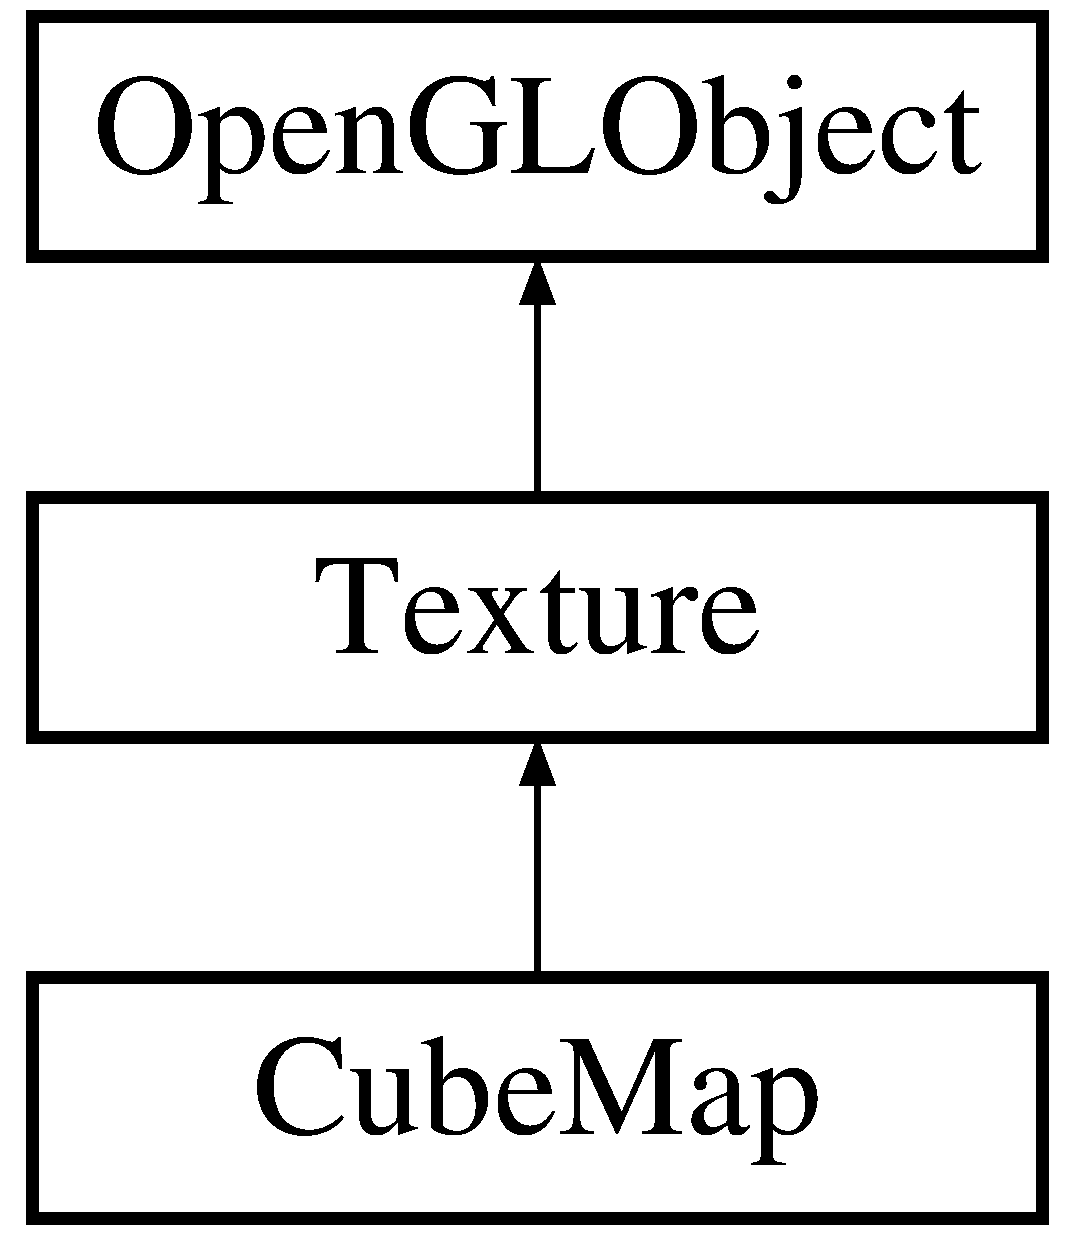
\includegraphics[height=3.000000cm]{class_cube_map}
\end{center}
\end{figure}
\subsection*{Public Member Functions}
\begin{DoxyCompactItemize}
\item 
void \hyperlink{class_cube_map_a0b1e25c2b88f8f32f4c137a8e0ca9cc2}{load} (const std\+::array$<$ std\+::string, 6 $>$ \&Paths)
\item 
\hypertarget{class_cube_map_ab2362f1c3487e918995adec3e6100762}{void {\bfseries create} (const std\+::array$<$ void $\ast$, 6 $>$ \&Data, size\+\_\+t width, size\+\_\+t height, int comp\+Count)}\label{class_cube_map_ab2362f1c3487e918995adec3e6100762}

\item 
\hypertarget{class_cube_map_acfaa0ac1c35bbbc0aa0ad7ab93b303c0}{void {\bfseries bind} (int Unit\+Texture=0) const }\label{class_cube_map_acfaa0ac1c35bbbc0aa0ad7ab93b303c0}

\end{DoxyCompactItemize}
\subsection*{Static Public Member Functions}
\begin{DoxyCompactItemize}
\item 
\hypertarget{class_cube_map_a744cf80626f1b59deb66077751e03083}{static void {\bfseries unbind} ()}\label{class_cube_map_a744cf80626f1b59deb66077751e03083}

\end{DoxyCompactItemize}
\subsection*{Additional Inherited Members}


\subsection{Member Function Documentation}
\hypertarget{class_cube_map_a0b1e25c2b88f8f32f4c137a8e0ca9cc2}{\index{Cube\+Map@{Cube\+Map}!load@{load}}
\index{load@{load}!Cube\+Map@{Cube\+Map}}
\subsubsection[{load}]{\setlength{\rightskip}{0pt plus 5cm}void Cube\+Map\+::load (
\begin{DoxyParamCaption}
\item[{const std\+::array$<$ std\+::string, 6 $>$ \&}]{Paths}
\end{DoxyParamCaption}
)}}\label{class_cube_map_a0b1e25c2b88f8f32f4c137a8e0ca9cc2}
Order \+: X\+P\+O\+S, X\+N\+E\+G, Y\+P\+O\+S, Y\+N\+E\+G, Z\+P\+O\+S, Z\+N\+E\+G 

The documentation for this class was generated from the following files\+:\begin{DoxyCompactItemize}
\item 
src/\+Graphics/Cube\+Map.\+hpp\item 
src/\+Graphics/Cube\+Map.\+cpp\end{DoxyCompactItemize}

\hypertarget{class_cubic_spline}{\section{Cubic\+Spline$<$ T, R $>$ Class Template Reference}
\label{class_cubic_spline}\index{Cubic\+Spline$<$ T, R $>$@{Cubic\+Spline$<$ T, R $>$}}
}


{\ttfamily \#include $<$Cubic\+Spline.\+hpp$>$}

\subsection*{Classes}
\begin{DoxyCompactItemize}
\item 
class \hyperlink{class_cubic_spline_1_1_control_point}{Control\+Point}
\end{DoxyCompactItemize}
\subsection*{Public Member Functions}
\begin{DoxyCompactItemize}
\item 
\hyperlink{class_cubic_spline_aa96fa0cae57adc1b3b54ba6c77449bf9}{Cubic\+Spline} ()=default
\item 
\hyperlink{class_cubic_spline_a7dda562cc8c8e21795fae07cd795e34f}{Cubic\+Spline} (const \hyperlink{class_cubic_spline}{Cubic\+Spline}$<$ T, R $>$ \&)=default
\item 
\hyperlink{class_cubic_spline_a60273994d7a74bd9b32710fe85930886}{Cubic\+Spline} (\hyperlink{class_cubic_spline}{Cubic\+Spline}$<$ T, R $>$ \&\&)=default
\item 
\hyperlink{class_cubic_spline_ada95f74924601a63f49e5a9750b26820}{Cubic\+Spline} (const std\+::initializer\+\_\+list$<$ T $>$ \&L)
\item 
\hyperlink{class_cubic_spline_a1585facd63ce5a5a6d792bb74e463530}{Cubic\+Spline} (const std\+::initializer\+\_\+list$<$ \hyperlink{class_cubic_spline_1_1_control_point}{Control\+Point} $>$ \&L)
\item 
{\footnotesize template$<$class Iterator $>$ }\\\hyperlink{class_cubic_spline_a0b0fb22f91f159696773a7c9886917d3}{Cubic\+Spline} (Iterator Begin, Iterator End)
\item 
\hypertarget{class_cubic_spline_a63b02c717562f6188361d1cef7de36a0}{\hyperlink{class_cubic_spline}{Cubic\+Spline} \& {\bfseries operator=} (const \hyperlink{class_cubic_spline}{Cubic\+Spline} \&)=default}\label{class_cubic_spline_a63b02c717562f6188361d1cef7de36a0}

\item 
\hypertarget{class_cubic_spline_a6611d30ab9e2bc9da998da7284cde8a9}{\hyperlink{class_cubic_spline}{Cubic\+Spline} \& {\bfseries operator=} (\hyperlink{class_cubic_spline}{Cubic\+Spline} \&\&)=default}\label{class_cubic_spline_a6611d30ab9e2bc9da998da7284cde8a9}

\item 
\hypertarget{class_cubic_spline_a4b74494e4824a178cc6ee4af3bf4e6d0}{size\+\_\+t {\bfseries get\+Point\+Count} () const }\label{class_cubic_spline_a4b74494e4824a178cc6ee4af3bf4e6d0}

\item 
\hypertarget{class_cubic_spline_a0d6abd3a3216bb408d9623795633c291}{void {\bfseries operator+=} (const \hyperlink{class_cubic_spline_1_1_control_point}{Control\+Point} \&C)}\label{class_cubic_spline_a0d6abd3a3216bb408d9623795633c291}

\item 
\hypertarget{class_cubic_spline_acdf11d783a0dd7617a102da6eed6f2f7}{void {\bfseries add} (const \hyperlink{class_cubic_spline_1_1_control_point}{Control\+Point} \&C)}\label{class_cubic_spline_acdf11d783a0dd7617a102da6eed6f2f7}

\item 
\hypertarget{class_cubic_spline_ae588b1125265af223147542c2ea4a321}{R {\bfseries get\+Start\+Time} () const }\label{class_cubic_spline_ae588b1125265af223147542c2ea4a321}

\item 
\hypertarget{class_cubic_spline_a42c5272bdcc5e87703ae92f09f84d6ee}{R {\bfseries get\+End\+Time} () const }\label{class_cubic_spline_a42c5272bdcc5e87703ae92f09f84d6ee}

\item 
\hypertarget{class_cubic_spline_ac9e8435d327ccae34a5669ab521c89ab}{T {\bfseries operator()} (R t)}\label{class_cubic_spline_ac9e8435d327ccae34a5669ab521c89ab}

\item 
\hypertarget{class_cubic_spline_a9b3b37f8854ccb600a86143037968185}{T {\bfseries get} (R t)}\label{class_cubic_spline_a9b3b37f8854ccb600a86143037968185}

\item 
\hypertarget{class_cubic_spline_abbc03595baa0e3bbc6d9323156b036b6}{T {\bfseries get\+Speed} (R t)}\label{class_cubic_spline_abbc03595baa0e3bbc6d9323156b036b6}

\item 
\hypertarget{class_cubic_spline_aa90bb69636898cae50fa444178a1bb21}{T {\bfseries get\+Acceleration} (R t)}\label{class_cubic_spline_aa90bb69636898cae50fa444178a1bb21}

\item 
\hypertarget{class_cubic_spline_a721c7701df60b26a29ad0a8a161670a9}{void {\bfseries linear\+Timing} (R t=static\+\_\+cast$<$ R $>$(1.\+0))}\label{class_cubic_spline_a721c7701df60b26a29ad0a8a161670a9}

\item 
\hypertarget{class_cubic_spline_a7a7893b6a340d6d92d2f485050a8a177}{void {\bfseries catmull\+Rom} ()}\label{class_cubic_spline_a7a7893b6a340d6d92d2f485050a8a177}

\item 
\hypertarget{class_cubic_spline_a33beb7f9777ad224b90724d897a785d7}{std\+::vector$<$ \hyperlink{class_cubic_spline_1_1_control_point}{Control\+Point} $>$\\*
\+::iterator {\bfseries begin} ()}\label{class_cubic_spline_a33beb7f9777ad224b90724d897a785d7}

\item 
\hypertarget{class_cubic_spline_af2d1718c8f709bded0f22211ce5bdcbb}{std\+::vector$<$ \hyperlink{class_cubic_spline_1_1_control_point}{Control\+Point} $>$\\*
\+::iterator {\bfseries end} ()}\label{class_cubic_spline_af2d1718c8f709bded0f22211ce5bdcbb}

\item 
\hypertarget{class_cubic_spline_a29a317e8ea68912e4a6aa8e038441437}{std\+::vector$<$ \hyperlink{class_cubic_spline_1_1_control_point}{Control\+Point} $>$\\*
\+::const\+\_\+iterator {\bfseries begin} () const }\label{class_cubic_spline_a29a317e8ea68912e4a6aa8e038441437}

\item 
\hypertarget{class_cubic_spline_a004685a928570acac100be18fe42b4fe}{std\+::vector$<$ \hyperlink{class_cubic_spline_1_1_control_point}{Control\+Point} $>$\\*
\+::const\+\_\+iterator {\bfseries end} () const }\label{class_cubic_spline_a004685a928570acac100be18fe42b4fe}

\end{DoxyCompactItemize}


\subsection{Detailed Description}
\subsubsection*{template$<$class T, typename R = float$>$class Cubic\+Spline$<$ T, R $>$}

\hyperlink{class_cubic_spline}{Cubic\+Spline} Describes a \hyperlink{class_cubic_spline}{Cubic\+Spline} defined by Control\+Points. Each \hyperlink{class_cubic_spline_1_1_control_point}{Control\+Point} consist of at least a position, and optionally a speed (tangent) and a time (these two can be set to default values, giving you a \mbox{[}0, 1\mbox{]} catmull-\/rom spline).

\begin{DoxyRefDesc}{Todo}
\item[\hyperlink{todo__todo000001}{Todo}]Easier point insertion ? Auto sorting if time is specified ? 

Comment the whole thing\end{DoxyRefDesc}



\begin{DoxyParams}{Parameters}
{\em T} & Well defined vector class (addition, multiplication whith a scalar R) \\
\hline
{\em R} & Scalar type of the vector class (default\+: float) \\
\hline
\end{DoxyParams}


\subsection{Constructor \& Destructor Documentation}
\hypertarget{class_cubic_spline_aa96fa0cae57adc1b3b54ba6c77449bf9}{\index{Cubic\+Spline@{Cubic\+Spline}!Cubic\+Spline@{Cubic\+Spline}}
\index{Cubic\+Spline@{Cubic\+Spline}!Cubic\+Spline@{Cubic\+Spline}}
\subsubsection[{Cubic\+Spline}]{\setlength{\rightskip}{0pt plus 5cm}template$<$class T , typename R  = float$>$ {\bf Cubic\+Spline}$<$ T, R $>$\+::{\bf Cubic\+Spline} (
\begin{DoxyParamCaption}
{}
\end{DoxyParamCaption}
)\hspace{0.3cm}{\ttfamily [default]}}}\label{class_cubic_spline_aa96fa0cae57adc1b3b54ba6c77449bf9}
Default Constructor \hypertarget{class_cubic_spline_a7dda562cc8c8e21795fae07cd795e34f}{\index{Cubic\+Spline@{Cubic\+Spline}!Cubic\+Spline@{Cubic\+Spline}}
\index{Cubic\+Spline@{Cubic\+Spline}!Cubic\+Spline@{Cubic\+Spline}}
\subsubsection[{Cubic\+Spline}]{\setlength{\rightskip}{0pt plus 5cm}template$<$class T , typename R  = float$>$ {\bf Cubic\+Spline}$<$ T, R $>$\+::{\bf Cubic\+Spline} (
\begin{DoxyParamCaption}
\item[{const {\bf Cubic\+Spline}$<$ T, R $>$ \&}]{}
\end{DoxyParamCaption}
)\hspace{0.3cm}{\ttfamily [default]}}}\label{class_cubic_spline_a7dda562cc8c8e21795fae07cd795e34f}
Copy Constructor \hypertarget{class_cubic_spline_a60273994d7a74bd9b32710fe85930886}{\index{Cubic\+Spline@{Cubic\+Spline}!Cubic\+Spline@{Cubic\+Spline}}
\index{Cubic\+Spline@{Cubic\+Spline}!Cubic\+Spline@{Cubic\+Spline}}
\subsubsection[{Cubic\+Spline}]{\setlength{\rightskip}{0pt plus 5cm}template$<$class T , typename R  = float$>$ {\bf Cubic\+Spline}$<$ T, R $>$\+::{\bf Cubic\+Spline} (
\begin{DoxyParamCaption}
\item[{{\bf Cubic\+Spline}$<$ T, R $>$ \&\&}]{}
\end{DoxyParamCaption}
)\hspace{0.3cm}{\ttfamily [default]}}}\label{class_cubic_spline_a60273994d7a74bd9b32710fe85930886}
Move Constructor \hypertarget{class_cubic_spline_ada95f74924601a63f49e5a9750b26820}{\index{Cubic\+Spline@{Cubic\+Spline}!Cubic\+Spline@{Cubic\+Spline}}
\index{Cubic\+Spline@{Cubic\+Spline}!Cubic\+Spline@{Cubic\+Spline}}
\subsubsection[{Cubic\+Spline}]{\setlength{\rightskip}{0pt plus 5cm}template$<$class T , typename R  = float$>$ {\bf Cubic\+Spline}$<$ T, R $>$\+::{\bf Cubic\+Spline} (
\begin{DoxyParamCaption}
\item[{const std\+::initializer\+\_\+list$<$ T $>$ \&}]{L}
\end{DoxyParamCaption}
)}}\label{class_cubic_spline_ada95f74924601a63f49e5a9750b26820}
Constructor by list of positions \hypertarget{class_cubic_spline_a1585facd63ce5a5a6d792bb74e463530}{\index{Cubic\+Spline@{Cubic\+Spline}!Cubic\+Spline@{Cubic\+Spline}}
\index{Cubic\+Spline@{Cubic\+Spline}!Cubic\+Spline@{Cubic\+Spline}}
\subsubsection[{Cubic\+Spline}]{\setlength{\rightskip}{0pt plus 5cm}template$<$class T , typename R  = float$>$ {\bf Cubic\+Spline}$<$ T, R $>$\+::{\bf Cubic\+Spline} (
\begin{DoxyParamCaption}
\item[{const std\+::initializer\+\_\+list$<$ {\bf Control\+Point} $>$ \&}]{L}
\end{DoxyParamCaption}
)}}\label{class_cubic_spline_a1585facd63ce5a5a6d792bb74e463530}
Constructor by list of Control\+Points \hypertarget{class_cubic_spline_a0b0fb22f91f159696773a7c9886917d3}{\index{Cubic\+Spline@{Cubic\+Spline}!Cubic\+Spline@{Cubic\+Spline}}
\index{Cubic\+Spline@{Cubic\+Spline}!Cubic\+Spline@{Cubic\+Spline}}
\subsubsection[{Cubic\+Spline}]{\setlength{\rightskip}{0pt plus 5cm}template$<$class T , typename R  = float$>$ template$<$class Iterator $>$ {\bf Cubic\+Spline}$<$ T, R $>$\+::{\bf Cubic\+Spline} (
\begin{DoxyParamCaption}
\item[{Iterator}]{Begin, }
\item[{Iterator}]{End}
\end{DoxyParamCaption}
)}}\label{class_cubic_spline_a0b0fb22f91f159696773a7c9886917d3}
Constructor by list of positions 

The documentation for this class was generated from the following file\+:\begin{DoxyCompactItemize}
\item 
src/Cubic\+Spline.\+hpp\end{DoxyCompactItemize}

\hypertarget{class_curve}{\section{Curve$<$ T, R $>$ Class Template Reference}
\label{class_curve}\index{Curve$<$ T, R $>$@{Curve$<$ T, R $>$}}
}
Inheritance diagram for Curve$<$ T, R $>$\+:\begin{figure}[H]
\begin{center}
\leavevmode
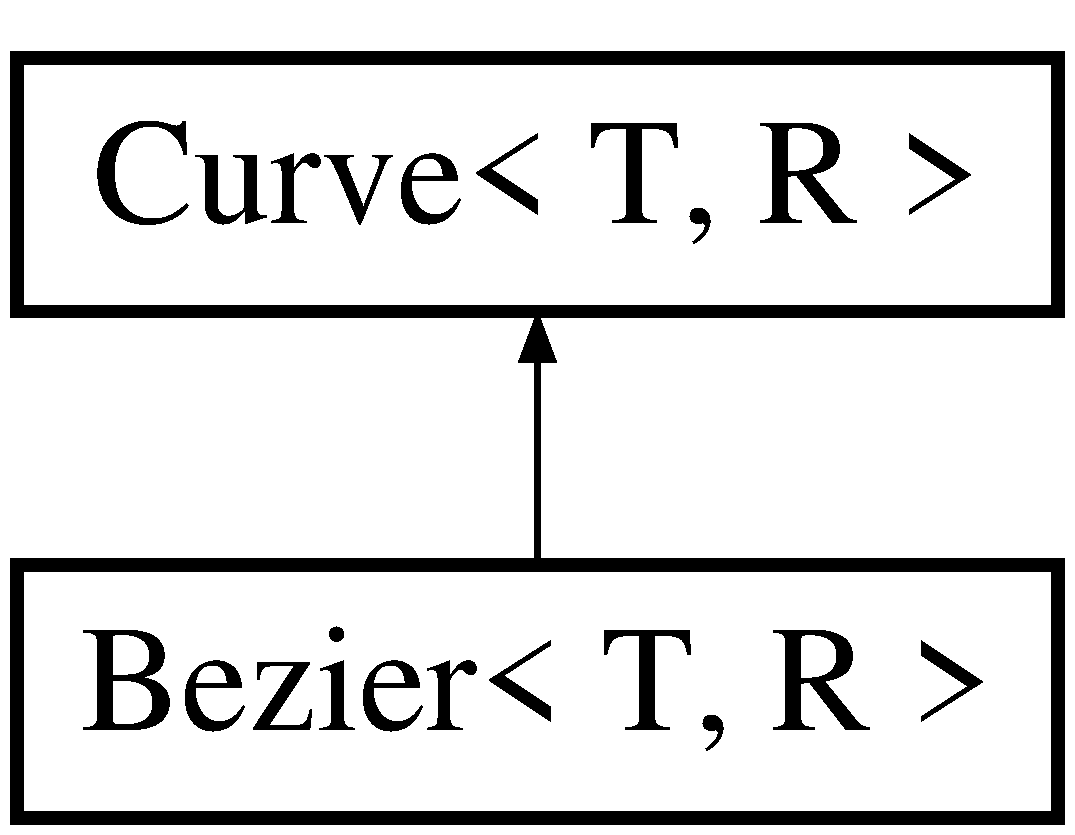
\includegraphics[height=2.000000cm]{class_curve}
\end{center}
\end{figure}
\subsection*{Public Member Functions}
\begin{DoxyCompactItemize}
\item 
\hypertarget{class_curve_acf1a8243f5866354dc219de4e46812f1}{{\bfseries Curve} (const \hyperlink{class_curve}{Curve}$<$ T, R $>$ \&)=default}\label{class_curve_acf1a8243f5866354dc219de4e46812f1}

\item 
\hypertarget{class_curve_aad4e437b4852e30ff80795bc26bf6acc}{{\bfseries Curve} (\hyperlink{class_curve}{Curve}$<$ T, R $>$ \&\&)=default}\label{class_curve_aad4e437b4852e30ff80795bc26bf6acc}

\item 
\hypertarget{class_curve_ac44599de71da0036206bc3c394718982}{{\bfseries Curve} (const std\+::initializer\+\_\+list$<$ T $>$ \&L)}\label{class_curve_ac44599de71da0036206bc3c394718982}

\item 
\hypertarget{class_curve_a12df06dd0d0bd6057df64ab7adcf7f87}{{\footnotesize template$<$class Iterator $>$ }\\{\bfseries Curve} (Iterator Begin, Iterator End)}\label{class_curve_a12df06dd0d0bd6057df64ab7adcf7f87}

\item 
\hypertarget{class_curve_a1f5d904ae8065ce84bed3b35a6c986fc}{\hyperlink{class_curve}{Curve} \& {\bfseries operator=} (const \hyperlink{class_curve}{Curve} \&)=default}\label{class_curve_a1f5d904ae8065ce84bed3b35a6c986fc}

\item 
\hypertarget{class_curve_a3513c7344f57c252d4e26d08d5443065}{\hyperlink{class_curve}{Curve} \& {\bfseries operator=} (\hyperlink{class_curve}{Curve} \&\&)=default}\label{class_curve_a3513c7344f57c252d4e26d08d5443065}

\item 
\hypertarget{class_curve_a3f1470b2c32786ee3377890c96d0aa26}{size\+\_\+t {\bfseries get\+Point\+Count} () const }\label{class_curve_a3f1470b2c32786ee3377890c96d0aa26}

\item 
\hypertarget{class_curve_a2c34dfe2f8ee8a81b6fa7321600f12ba}{const T \& {\bfseries operator\mbox{[}$\,$\mbox{]}} (size\+\_\+t idx) const }\label{class_curve_a2c34dfe2f8ee8a81b6fa7321600f12ba}

\item 
\hypertarget{class_curve_ac090e6c8c54c80d4488a6dca7137a53f}{\hyperlink{class_curve}{Curve} \& {\bfseries operator+=} (const T \&P)}\label{class_curve_ac090e6c8c54c80d4488a6dca7137a53f}

\item 
virtual T \hyperlink{class_curve_a1ba9ed5a0a932891bce8959f4bc0d472}{get} (R t) const 
\begin{DoxyCompactList}\small\item\em Compute the approximate value of the curve at t. \end{DoxyCompactList}\item 
\hypertarget{class_curve_a15b3d5628157bebb61b5dadc90754808}{std\+::vector$<$ T $>$\+::iterator {\bfseries begin} ()}\label{class_curve_a15b3d5628157bebb61b5dadc90754808}

\item 
\hypertarget{class_curve_ab1aacb0bf268c08899e9f3682354bcbc}{std\+::vector$<$ T $>$\+::iterator {\bfseries end} ()}\label{class_curve_ab1aacb0bf268c08899e9f3682354bcbc}

\item 
\hypertarget{class_curve_a8b25460468341733b1429002bb86ec16}{std\+::vector$<$ T $>$\+::const\+\_\+iterator {\bfseries begin} () const }\label{class_curve_a8b25460468341733b1429002bb86ec16}

\item 
\hypertarget{class_curve_ac998e899d27c4786761fc41a9ad0623e}{std\+::vector$<$ T $>$\+::const\+\_\+iterator {\bfseries end} () const }\label{class_curve_ac998e899d27c4786761fc41a9ad0623e}

\end{DoxyCompactItemize}
\subsection*{Protected Attributes}
\begin{DoxyCompactItemize}
\item 
\hypertarget{class_curve_a7cf738991496191e81517ad930dc2528}{std\+::vector$<$ T $>$ {\bfseries \+\_\+points}}\label{class_curve_a7cf738991496191e81517ad930dc2528}

\end{DoxyCompactItemize}


\subsection{Member Function Documentation}
\hypertarget{class_curve_a1ba9ed5a0a932891bce8959f4bc0d472}{\index{Curve@{Curve}!get@{get}}
\index{get@{get}!Curve@{Curve}}
\subsubsection[{get}]{\setlength{\rightskip}{0pt plus 5cm}template$<$class T, typename R = float$>$ virtual T {\bf Curve}$<$ T, R $>$\+::get (
\begin{DoxyParamCaption}
\item[{R}]{t}
\end{DoxyParamCaption}
) const\hspace{0.3cm}{\ttfamily [inline]}, {\ttfamily [virtual]}}}\label{class_curve_a1ba9ed5a0a932891bce8959f4bc0d472}


Compute the approximate value of the curve at t. 


\begin{DoxyParams}{Parameters}
{\em t} & 0.\+f $<$= t $<$= 1.\+0f \\
\hline
\end{DoxyParams}


The documentation for this class was generated from the following file\+:\begin{DoxyCompactItemize}
\item 
src/Curve.\+hpp\end{DoxyCompactItemize}

\hypertarget{class_fragment_shader}{\section{Fragment\+Shader Class Reference}
\label{class_fragment_shader}\index{Fragment\+Shader@{Fragment\+Shader}}
}
Inheritance diagram for Fragment\+Shader\+:\begin{figure}[H]
\begin{center}
\leavevmode
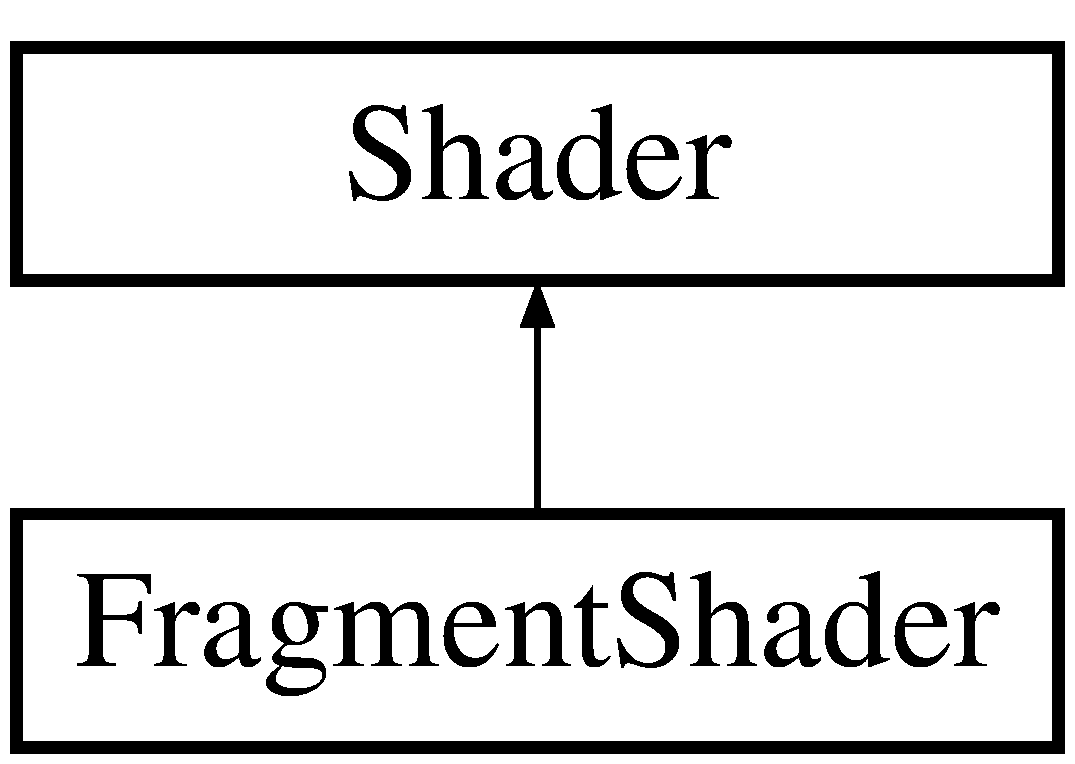
\includegraphics[height=2.000000cm]{class_fragment_shader}
\end{center}
\end{figure}
\subsection*{Additional Inherited Members}


The documentation for this class was generated from the following files\+:\begin{DoxyCompactItemize}
\item 
src/\+Graphics/\+Shader\+Program/Fragment\+Shader.\+hpp\item 
src/\+Graphics/\+Shader\+Program/Fragment\+Shader.\+cpp\end{DoxyCompactItemize}

\hypertarget{class_framebuffer}{\section{Framebuffer$<$ Tex\+Type $>$ Class Template Reference}
\label{class_framebuffer}\index{Framebuffer$<$ Tex\+Type $>$@{Framebuffer$<$ Tex\+Type $>$}}
}
Inheritance diagram for Framebuffer$<$ Tex\+Type $>$\+:\begin{figure}[H]
\begin{center}
\leavevmode
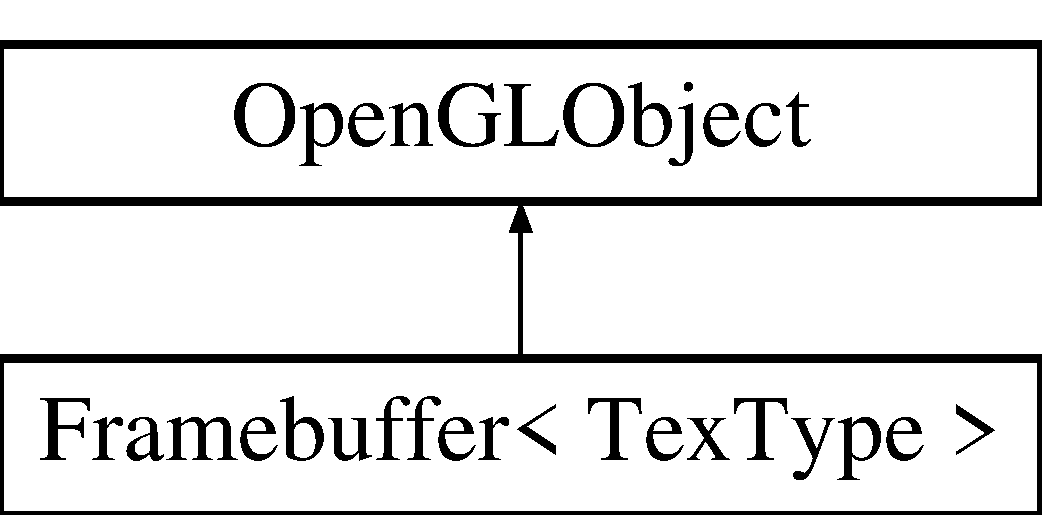
\includegraphics[height=2.000000cm]{class_framebuffer}
\end{center}
\end{figure}
\subsection*{Public Member Functions}
\begin{DoxyCompactItemize}
\item 
\hypertarget{class_framebuffer_af1dca358cc28fcd088cddec942c06f81}{{\bfseries Framebuffer} (size\+\_\+t size=512, bool use\+Depth=true)}\label{class_framebuffer_af1dca358cc28fcd088cddec942c06f81}

\item 
\hypertarget{class_framebuffer_a2c7588cabdab14126f3979a1eb6bc0a4}{{\bfseries Framebuffer} (size\+\_\+t width, size\+\_\+t height, bool use\+Depth=true)}\label{class_framebuffer_a2c7588cabdab14126f3979a1eb6bc0a4}

\item 
\hypertarget{class_framebuffer_aba8bd86011c1d69e71a5484385e25612}{virtual void {\bfseries init} ()}\label{class_framebuffer_aba8bd86011c1d69e71a5484385e25612}

\item 
\hypertarget{class_framebuffer_a2d5e250c6cf94ccd1347451388711851}{void {\bfseries bind} (G\+Lenum target=G\+L\+\_\+\+F\+R\+A\+M\+E\+B\+U\+F\+F\+E\+R) const }\label{class_framebuffer_a2d5e250c6cf94ccd1347451388711851}

\item 
\hypertarget{class_framebuffer_a8eb942266a2b5fb870b0d938d87141b2}{Tex\+Type \& {\bfseries get\+Color} ()}\label{class_framebuffer_a8eb942266a2b5fb870b0d938d87141b2}

\item 
\hypertarget{class_framebuffer_aa617cd6ac95905c23636d42439e6191b}{Tex\+Type \& {\bfseries get\+Depth} ()}\label{class_framebuffer_aa617cd6ac95905c23636d42439e6191b}

\end{DoxyCompactItemize}
\subsection*{Static Public Member Functions}
\begin{DoxyCompactItemize}
\item 
\hypertarget{class_framebuffer_a9d8decc066a570ebc86567c2adb17530}{static void {\bfseries unbind} (G\+Lenum target=G\+L\+\_\+\+F\+R\+A\+M\+E\+B\+U\+F\+F\+E\+R)}\label{class_framebuffer_a9d8decc066a570ebc86567c2adb17530}

\end{DoxyCompactItemize}


The documentation for this class was generated from the following file\+:\begin{DoxyCompactItemize}
\item 
src/\+Graphics/Framebuffer.\+hpp\end{DoxyCompactItemize}

\hypertarget{class_framebuffer_3_01_cube_map_01_4}{\section{Framebuffer$<$ Cube\+Map $>$ Class Template Reference}
\label{class_framebuffer_3_01_cube_map_01_4}\index{Framebuffer$<$ Cube\+Map $>$@{Framebuffer$<$ Cube\+Map $>$}}
}
\subsection*{Public Member Functions}
\begin{DoxyCompactItemize}
\item 
\hypertarget{class_framebuffer_3_01_cube_map_01_4_a4f2023ad456a8e264228994305367772}{{\bfseries Framebuffer} (size\+\_\+t size=512)}\label{class_framebuffer_3_01_cube_map_01_4_a4f2023ad456a8e264228994305367772}

\item 
\hypertarget{class_framebuffer_3_01_cube_map_01_4_a78ee821aa870f0b1a20037b3fef93440}{void {\bfseries init} ()}\label{class_framebuffer_3_01_cube_map_01_4_a78ee821aa870f0b1a20037b3fef93440}

\item 
\hypertarget{class_framebuffer_3_01_cube_map_01_4_a8af2dea06f02f1006e9a2464de4781c6}{void {\bfseries bind} (G\+Lenum target=G\+L\+\_\+\+D\+R\+A\+W\+\_\+\+F\+R\+A\+M\+E\+B\+U\+F\+F\+E\+R)}\label{class_framebuffer_3_01_cube_map_01_4_a8af2dea06f02f1006e9a2464de4781c6}

\item 
\hypertarget{class_framebuffer_3_01_cube_map_01_4_a13f90271d17e9044ee8a6b9851e23cad}{\hyperlink{class_cube_map}{Cube\+Map} \& {\bfseries get\+Color\+Cubemap} ()}\label{class_framebuffer_3_01_cube_map_01_4_a13f90271d17e9044ee8a6b9851e23cad}

\item 
\hypertarget{class_framebuffer_3_01_cube_map_01_4_a030db738a715d191b44364bfb2bff900}{\hyperlink{class_cube_map}{Cube\+Map} \& {\bfseries get\+Depth\+Cubemap} ()}\label{class_framebuffer_3_01_cube_map_01_4_a030db738a715d191b44364bfb2bff900}

\end{DoxyCompactItemize}
\subsection*{Static Public Member Functions}
\begin{DoxyCompactItemize}
\item 
\hypertarget{class_framebuffer_3_01_cube_map_01_4_abeacf4f546f7eacccf0c84e348ebd9bc}{static void {\bfseries unbind} (G\+Lenum target=G\+L\+\_\+\+D\+R\+A\+W\+\_\+\+F\+R\+A\+M\+E\+B\+U\+F\+F\+E\+R)}\label{class_framebuffer_3_01_cube_map_01_4_abeacf4f546f7eacccf0c84e348ebd9bc}

\end{DoxyCompactItemize}


The documentation for this class was generated from the following file\+:\begin{DoxyCompactItemize}
\item 
src/\+Graphics/Cube\+Framebuffer.\+hpp\end{DoxyCompactItemize}

\hypertarget{class_frustum}{\section{Frustum Class Reference}
\label{class_frustum}\index{Frustum@{Frustum}}
}
\subsection*{Public Types}
\begin{DoxyCompactItemize}
\item 
\hypertarget{class_frustum_ace19a96bed0212d446a02991b336d50d}{enum {\bfseries Face} \{ \\*
{\bfseries Top}, 
{\bfseries Bottom}, 
{\bfseries Left}, 
{\bfseries Right}, 
\\*
{\bfseries Near}, 
{\bfseries Far}
 \}}\label{class_frustum_ace19a96bed0212d446a02991b336d50d}

\end{DoxyCompactItemize}
\subsection*{Public Member Functions}
\begin{DoxyCompactItemize}
\item 
\hypertarget{class_frustum_a324d013a34add360bbf8a6eb4b095549}{void {\bfseries set\+Perspective} (float angle, float ratio, float znear, float zfar)}\label{class_frustum_a324d013a34add360bbf8a6eb4b095549}

\item 
\hypertarget{class_frustum_a329f42eec391f45fae390b10483ff9eb}{void \hyperlink{class_frustum_a329f42eec391f45fae390b10483ff9eb}{set\+Look\+At} (const glm\+::vec3 \&pos, const glm\+::vec3 \&dir, const glm\+::vec3 \&up)}\label{class_frustum_a329f42eec391f45fae390b10483ff9eb}

\begin{DoxyCompactList}\small\item\em Testing against a sphere. \end{DoxyCompactList}\item 
\hypertarget{class_frustum_aaf2fcddd7f6105e303f110f2a4ecac1b}{bool \hyperlink{class_frustum_aaf2fcddd7f6105e303f110f2a4ecac1b}{is\+Intersecting} (const glm\+::vec3 \&center, float radius) const }\label{class_frustum_aaf2fcddd7f6105e303f110f2a4ecac1b}

\begin{DoxyCompactList}\small\item\em Testing against a sphere. \end{DoxyCompactList}\item 
\hypertarget{class_frustum_a478873b2d524b3e282fc0bdd6f63d320}{bool {\bfseries changed} ()}\label{class_frustum_a478873b2d524b3e282fc0bdd6f63d320}

\end{DoxyCompactItemize}


The documentation for this class was generated from the following files\+:\begin{DoxyCompactItemize}
\item 
src/\+Graphics/Frustum.\+hpp\item 
src/\+Graphics/Frustum.\+cpp\end{DoxyCompactItemize}

\hypertarget{class_generic_uniform}{\section{Generic\+Uniform Class Reference}
\label{class_generic_uniform}\index{Generic\+Uniform@{Generic\+Uniform}}
}
Inheritance diagram for Generic\+Uniform\+:\begin{figure}[H]
\begin{center}
\leavevmode
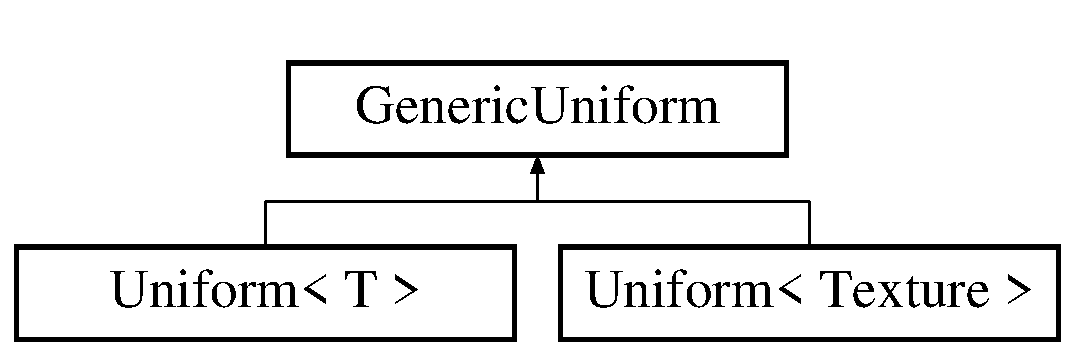
\includegraphics[height=2.000000cm]{class_generic_uniform}
\end{center}
\end{figure}
\subsection*{Public Member Functions}
\begin{DoxyCompactItemize}
\item 
\hypertarget{class_generic_uniform_a0779c308a727477f24e384c49184ab21}{{\bfseries Generic\+Uniform} (const std\+::string \&N, G\+Luint L)}\label{class_generic_uniform_a0779c308a727477f24e384c49184ab21}

\item 
\hypertarget{class_generic_uniform_a86859a4955ece317e6ed9a72383b71f7}{const std\+::string \& {\bfseries get\+Name} () const }\label{class_generic_uniform_a86859a4955ece317e6ed9a72383b71f7}

\item 
\hypertarget{class_generic_uniform_aecd6e3593e457da2904091520309c8c8}{G\+Luint {\bfseries get\+Location} () const }\label{class_generic_uniform_aecd6e3593e457da2904091520309c8c8}

\item 
\hypertarget{class_generic_uniform_a7059915d2276ddcc2343b2d88c55ae2a}{void {\bfseries set\+Location} (const G\+Luint val)}\label{class_generic_uniform_a7059915d2276ddcc2343b2d88c55ae2a}

\end{DoxyCompactItemize}


The documentation for this class was generated from the following file\+:\begin{DoxyCompactItemize}
\item 
src/\+Graphics/\+Shader\+Program/\+W\+I\+P/Uniform.\+hpp\end{DoxyCompactItemize}

\hypertarget{class_geometry_shader}{\section{Geometry\+Shader Class Reference}
\label{class_geometry_shader}\index{Geometry\+Shader@{Geometry\+Shader}}
}
Inheritance diagram for Geometry\+Shader\+:\begin{figure}[H]
\begin{center}
\leavevmode
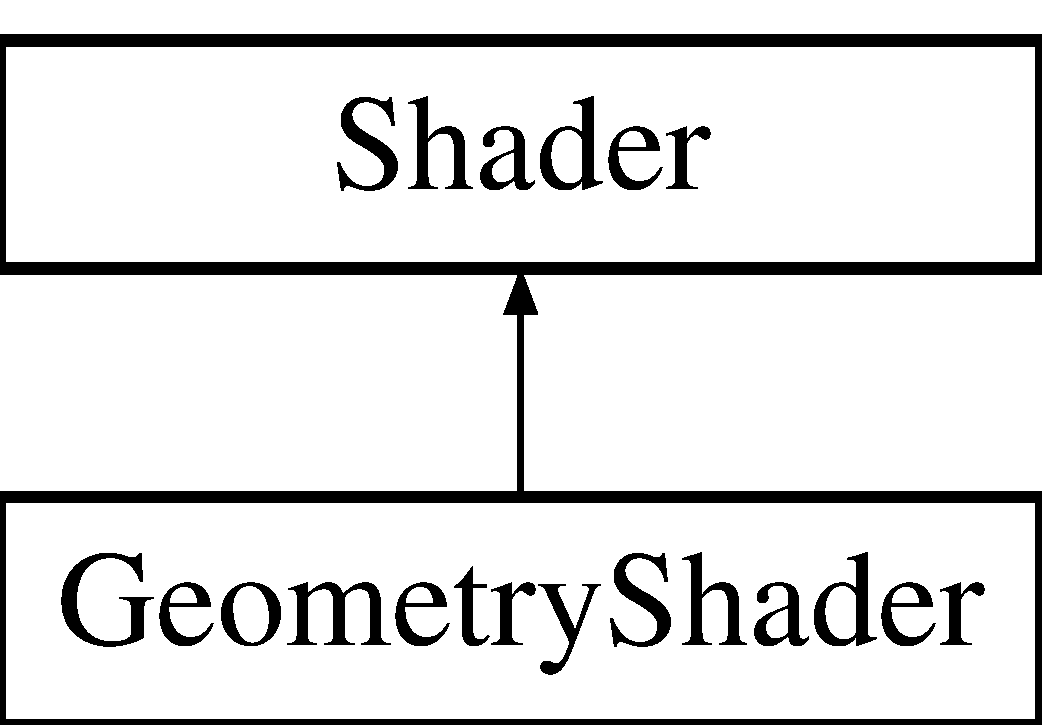
\includegraphics[height=2.000000cm]{class_geometry_shader}
\end{center}
\end{figure}
\subsection*{Additional Inherited Members}


The documentation for this class was generated from the following files\+:\begin{DoxyCompactItemize}
\item 
src/\+Graphics/\+Shader\+Program/Geometry\+Shader.\+hpp\item 
src/\+Graphics/\+Shader\+Program/Geometry\+Shader.\+cpp\end{DoxyCompactItemize}

\hypertarget{structhuffman}{\section{huffman Struct Reference}
\label{structhuffman}\index{huffman@{huffman}}
}
\subsection*{Public Attributes}
\begin{DoxyCompactItemize}
\item 
\hypertarget{structhuffman_a9dbb29a8ed724a32f502d9595510ddc2}{uint8 {\bfseries fast} \mbox{[}1$<$$<$ F\+A\+S\+T\+\_\+\+B\+I\+T\+S\mbox{]}}\label{structhuffman_a9dbb29a8ed724a32f502d9595510ddc2}

\item 
\hypertarget{structhuffman_a9925018a95d5a2122cd732561fa0fa64}{uint16 {\bfseries code} \mbox{[}256\mbox{]}}\label{structhuffman_a9925018a95d5a2122cd732561fa0fa64}

\item 
\hypertarget{structhuffman_a313d78cf23f40b314c25681ff2a6224b}{uint8 {\bfseries values} \mbox{[}256\mbox{]}}\label{structhuffman_a313d78cf23f40b314c25681ff2a6224b}

\item 
\hypertarget{structhuffman_afdb0fbcf25aec42ba30b0d0e2453a057}{uint8 {\bfseries size} \mbox{[}257\mbox{]}}\label{structhuffman_afdb0fbcf25aec42ba30b0d0e2453a057}

\item 
\hypertarget{structhuffman_aeb78aca6c7377faaad8123566d54fc98}{unsigned int {\bfseries maxcode} \mbox{[}18\mbox{]}}\label{structhuffman_aeb78aca6c7377faaad8123566d54fc98}

\item 
\hypertarget{structhuffman_a04255e3e1c6de74d36a08a1aa4e9537d}{int {\bfseries delta} \mbox{[}17\mbox{]}}\label{structhuffman_a04255e3e1c6de74d36a08a1aa4e9537d}

\end{DoxyCompactItemize}


The documentation for this struct was generated from the following file\+:\begin{DoxyCompactItemize}
\item 
src/\+Graphics/stb\+\_\+image.\+cpp\end{DoxyCompactItemize}

\hypertarget{structjpeg}{\section{jpeg Struct Reference}
\label{structjpeg}\index{jpeg@{jpeg}}
}
\subsection*{Public Attributes}
\begin{DoxyCompactItemize}
\item 
\hypertarget{structjpeg_aa1dac6b3ea069114abf0b4021aa3a67e}{\hyperlink{structstbi}{stbi} $\ast$ {\bfseries s}}\label{structjpeg_aa1dac6b3ea069114abf0b4021aa3a67e}

\item 
\hypertarget{structjpeg_aae44f91bafcc73fa70544573458abe33}{\hyperlink{structhuffman}{huffman} {\bfseries huff\+\_\+dc} \mbox{[}4\mbox{]}}\label{structjpeg_aae44f91bafcc73fa70544573458abe33}

\item 
\hypertarget{structjpeg_a6fab0b2d90425db5d609edbde8bddd92}{\hyperlink{structhuffman}{huffman} {\bfseries huff\+\_\+ac} \mbox{[}4\mbox{]}}\label{structjpeg_a6fab0b2d90425db5d609edbde8bddd92}

\item 
\hypertarget{structjpeg_aae820981dde2c49bc05b6e1298143d21}{uint8 {\bfseries dequant} \mbox{[}4\mbox{]}\mbox{[}64\mbox{]}}\label{structjpeg_aae820981dde2c49bc05b6e1298143d21}

\item 
\hypertarget{structjpeg_af4ed1173241e83f1482a276a178ce9e5}{int {\bfseries img\+\_\+h\+\_\+max}}\label{structjpeg_af4ed1173241e83f1482a276a178ce9e5}

\item 
\hypertarget{structjpeg_a50690c7d415968f864f4f1c10b85082d}{int {\bfseries img\+\_\+v\+\_\+max}}\label{structjpeg_a50690c7d415968f864f4f1c10b85082d}

\item 
\hypertarget{structjpeg_a8a7f2486617a69e9b88c9a161560c8a5}{int {\bfseries img\+\_\+mcu\+\_\+x}}\label{structjpeg_a8a7f2486617a69e9b88c9a161560c8a5}

\item 
\hypertarget{structjpeg_afa9d2c991eff0959c0c8b65ab186243b}{int {\bfseries img\+\_\+mcu\+\_\+y}}\label{structjpeg_afa9d2c991eff0959c0c8b65ab186243b}

\item 
\hypertarget{structjpeg_a32f06fea63ec2c976092760b21abad72}{int {\bfseries img\+\_\+mcu\+\_\+w}}\label{structjpeg_a32f06fea63ec2c976092760b21abad72}

\item 
\hypertarget{structjpeg_a6e013436253bcf1e5808a1774b96cc38}{int {\bfseries img\+\_\+mcu\+\_\+h}}\label{structjpeg_a6e013436253bcf1e5808a1774b96cc38}

\item 
\hypertarget{structjpeg_adeea25d03df153b0da048bea89b5c8b3}{\begin{tabbing}
xx\=xx\=xx\=xx\=xx\=xx\=xx\=xx\=xx\=\kill
struct \{\\
\>int {\bfseries id}\\
\>int {\bfseries h}\\
\>int {\bfseries v}\\
\>int {\bfseries tq}\\
\>int {\bfseries hd}\\
\>int {\bfseries ha}\\
\>int {\bfseries dc\_pred}\\
\>int {\bfseries x}\\
\>int {\bfseries y}\\
\>int {\bfseries w2}\\
\>int {\bfseries h2}\\
\>uint8 $\ast$ {\bfseries data}\\
\>void $\ast$ {\bfseries raw\_data}\\
\>uint8 $\ast$ {\bfseries linebuf}\\
\} {\bfseries img\_comp} \mbox{[}4\mbox{]}}\label{structjpeg_adeea25d03df153b0da048bea89b5c8b3}
\\

\end{tabbing}\item 
\hypertarget{structjpeg_abfc7f6a333ba3517e669e3e58113bbca}{uint32 {\bfseries code\+\_\+buffer}}\label{structjpeg_abfc7f6a333ba3517e669e3e58113bbca}

\item 
\hypertarget{structjpeg_a6d1b20b5d9d253006fde4e4dd8ab8c04}{int {\bfseries code\+\_\+bits}}\label{structjpeg_a6d1b20b5d9d253006fde4e4dd8ab8c04}

\item 
\hypertarget{structjpeg_a9a5cd40790fd432795fb19477c921f8c}{unsigned char {\bfseries marker}}\label{structjpeg_a9a5cd40790fd432795fb19477c921f8c}

\item 
\hypertarget{structjpeg_a2d114f4d52f50d8d85f43b2a3f161cec}{int {\bfseries nomore}}\label{structjpeg_a2d114f4d52f50d8d85f43b2a3f161cec}

\item 
\hypertarget{structjpeg_adca2f04da72e50086c77c7070731a679}{int {\bfseries scan\+\_\+n}}\label{structjpeg_adca2f04da72e50086c77c7070731a679}

\item 
\hypertarget{structjpeg_ac0f5240fc472e75239328f51a50f45b6}{int {\bfseries order} \mbox{[}4\mbox{]}}\label{structjpeg_ac0f5240fc472e75239328f51a50f45b6}

\item 
\hypertarget{structjpeg_ab13af34259b1f1c6cf8f35411a77e39e}{int {\bfseries restart\+\_\+interval}}\label{structjpeg_ab13af34259b1f1c6cf8f35411a77e39e}

\item 
\hypertarget{structjpeg_a6b4a8a352872847d84ea5ef1a4bc245e}{int {\bfseries todo}}\label{structjpeg_a6b4a8a352872847d84ea5ef1a4bc245e}

\end{DoxyCompactItemize}


The documentation for this struct was generated from the following file\+:\begin{DoxyCompactItemize}
\item 
src/\+Graphics/stb\+\_\+image.\+cpp\end{DoxyCompactItemize}

\hypertarget{class_light}{\section{Light Class Reference}
\label{class_light}\index{Light@{Light}}
}
\subsection*{Public Member Functions}
\begin{DoxyCompactItemize}
\item 
\hypertarget{class_light_a55223800cebd711b1f8e8b66c1472910}{void {\bfseries init} ()}\label{class_light_a55223800cebd711b1f8e8b66c1472910}

\end{DoxyCompactItemize}
\subsection*{Protected Attributes}
\begin{DoxyCompactItemize}
\item 
\hypertarget{class_light_ada9f418a6e3ab83806b9851956652d88}{glm\+::vec3 {\bfseries \+\_\+position} = glm\+::vec3(0.f)}\label{class_light_ada9f418a6e3ab83806b9851956652d88}

\item 
\hypertarget{class_light_aa6926e51bbb4185f7a4fe762215be877}{glm\+::vec3 {\bfseries \+\_\+direction} = glm\+::vec3(0.f, 0.f, 1.f)}\label{class_light_aa6926e51bbb4185f7a4fe762215be877}

\item 
\hypertarget{class_light_ad945d96eedca98e242b101b21bd2a8fc}{float {\bfseries \+\_\+range}}\label{class_light_ad945d96eedca98e242b101b21bd2a8fc}

\item 
\hypertarget{class_light_a7304a2765a5ccee487edef48041e6b2d}{glm\+::vec4 {\bfseries \+\_\+color} = glm\+::vec4(1.f)}\label{class_light_a7304a2765a5ccee487edef48041e6b2d}

\item 
\hypertarget{class_light_a898b7f4cee73c29894f2d1a26a170f48}{\hyperlink{class_frustum}{Frustum} {\bfseries \+\_\+frustum}}\label{class_light_a898b7f4cee73c29894f2d1a26a170f48}

\item 
\hypertarget{class_light_a6c324048008d9af8b1194f597c5fb755}{bool {\bfseries \+\_\+cast\+Shadows} = true}\label{class_light_a6c324048008d9af8b1194f597c5fb755}

\item 
\hypertarget{class_light_a311fcb523c9a0599cd898af1809e75f8}{unsigned int {\bfseries \+\_\+shadow\+Map\+Resolution} = 4096}\label{class_light_a311fcb523c9a0599cd898af1809e75f8}

\item 
\hypertarget{class_light_a2fb15f0412438f5a343bdb1557791689}{G\+Luint {\bfseries \+\_\+shadow\+Map\+Framebuffer} = 0}\label{class_light_a2fb15f0412438f5a343bdb1557791689}

\item 
\hypertarget{class_light_ae59a04ed9a1f1878bce9bfc0fa918f7e}{\hyperlink{class_texture}{Texture} {\bfseries \+\_\+shadow\+Map\+Depth\+Texture}}\label{class_light_ae59a04ed9a1f1878bce9bfc0fa918f7e}

\item 
\hypertarget{class_light_a1e5ea113e051058b583a4a97d0db42d2}{glm\+::mat4 {\bfseries \+\_\+depth\+Projection\+Matrix}}\label{class_light_a1e5ea113e051058b583a4a97d0db42d2}

\item 
\hypertarget{class_light_abc2190bf4f06b675021cfe25f1a8a38e}{glm\+::mat4 {\bfseries \+\_\+depth\+Bias\+M\+V\+P}}\label{class_light_abc2190bf4f06b675021cfe25f1a8a38e}

\end{DoxyCompactItemize}
\subsection*{Static Protected Attributes}
\begin{DoxyCompactItemize}
\item 
\hypertarget{class_light_aafd9db4848ed10a25adaa162559175a1}{static \hyperlink{class_program}{Program} \& {\bfseries \+\_\+depth\+Program}}\label{class_light_aafd9db4848ed10a25adaa162559175a1}

\item 
\hypertarget{class_light_a6e7e72476eb23068a660e499182e5dfa}{static \hyperlink{class_vertex_shader}{Vertex\+Shader} \& {\bfseries \+\_\+depth\+V\+S}}\label{class_light_a6e7e72476eb23068a660e499182e5dfa}

\item 
\hypertarget{class_light_a3a3c726b7846ccb2393740ed22878d13}{static \hyperlink{class_fragment_shader}{Fragment\+Shader} \& {\bfseries \+\_\+depth\+F\+S}}\label{class_light_a3a3c726b7846ccb2393740ed22878d13}

\end{DoxyCompactItemize}


The documentation for this class was generated from the following files\+:\begin{DoxyCompactItemize}
\item 
src/\+Graphics/Light.\+hpp\item 
src/\+Graphics/Light.\+cpp\end{DoxyCompactItemize}

\hypertarget{class_material}{\section{Material Class Reference}
\label{class_material}\index{Material@{Material}}
}
\subsection*{Classes}
\begin{DoxyCompactItemize}
\item 
class \hyperlink{class_material_1_1_uniform}{Uniform}
\end{DoxyCompactItemize}
\subsection*{Public Member Functions}
\begin{DoxyCompactItemize}
\item 
\hypertarget{class_material_a76819b8614c4184100af15ffcff511e8}{{\bfseries Material} (\hyperlink{class_program}{Program} \&P)}\label{class_material_a76819b8614c4184100af15ffcff511e8}

\item 
\hypertarget{class_material_a7ea61c71ac05b6df27fafa0ce2680341}{{\bfseries Material} (const \hyperlink{class_material}{Material} \&)=default}\label{class_material_a7ea61c71ac05b6df27fafa0ce2680341}

\item 
\hypertarget{class_material_ad097cc67cb4267568970a000adee3fcd}{\hyperlink{class_program}{Program} \& {\bfseries get\+Shading\+Program} ()}\label{class_material_ad097cc67cb4267568970a000adee3fcd}

\item 
\hypertarget{class_material_ae6b292382c0472f9a7317234dd7ec745}{void {\bfseries set\+Shading\+Program} (\hyperlink{class_program}{Program} \&P)}\label{class_material_ae6b292382c0472f9a7317234dd7ec745}

\item 
\hypertarget{class_material_a345766d313ba71edd8d20a3e44f41e0d}{void {\bfseries set\+Attribute} (const std\+::string \&Name, const float \&Value)}\label{class_material_a345766d313ba71edd8d20a3e44f41e0d}

\item 
\hypertarget{class_material_a64ef9d86ee8a2935a2c37ced96605b35}{void {\bfseries set\+Attribute} (const std\+::string \&Name, const int \&Value)}\label{class_material_a64ef9d86ee8a2935a2c37ced96605b35}

\item 
\hypertarget{class_material_a2efa2332318db2e2330bb30661d30fa2}{void {\bfseries set\+Attribute} (const std\+::string \&Name, const unsigned int \&Value)}\label{class_material_a2efa2332318db2e2330bb30661d30fa2}

\item 
\hypertarget{class_material_ab3c06a1202667f57b28212dd2d9d36dd}{void {\bfseries set\+Attribute} (const std\+::string \&Name, const glm\+::vec2 \&Value)}\label{class_material_ab3c06a1202667f57b28212dd2d9d36dd}

\item 
\hypertarget{class_material_a0f32aedf8001cf133879010b64f3fccd}{void {\bfseries set\+Attribute} (const std\+::string \&Name, const glm\+::vec3 \&Value)}\label{class_material_a0f32aedf8001cf133879010b64f3fccd}

\item 
\hypertarget{class_material_a08a66665e05d102fb5b0f2761ea93120}{void {\bfseries set\+Attribute} (const std\+::string \&Name, const glm\+::vec4 \&Value)}\label{class_material_a08a66665e05d102fb5b0f2761ea93120}

\item 
\hypertarget{class_material_afec72a611725bee8af7f3a3f1272bc7f}{void {\bfseries set\+Attribute} (const std\+::string \&Name, const glm\+::mat2 \&Value)}\label{class_material_afec72a611725bee8af7f3a3f1272bc7f}

\item 
\hypertarget{class_material_abba9a9832c1cf8feab2d81638340e2ff}{void {\bfseries set\+Attribute} (const std\+::string \&Name, const glm\+::mat3 \&Value)}\label{class_material_abba9a9832c1cf8feab2d81638340e2ff}

\item 
\hypertarget{class_material_a85e589886b3c6dd9e4dea1c2c70e1923}{void {\bfseries set\+Attribute} (const std\+::string \&Name, const glm\+::mat4 \&Value)}\label{class_material_a85e589886b3c6dd9e4dea1c2c70e1923}

\item 
\hypertarget{class_material_a8d121bc8fbc044b6b7525036df030389}{void {\bfseries set\+Attribute\+Ref} (const std\+::string \&Name, float \&Value)}\label{class_material_a8d121bc8fbc044b6b7525036df030389}

\item 
\hypertarget{class_material_a1ee0f946b87a4adb37b345e460f36d08}{void {\bfseries set\+Attribute\+Ref} (const std\+::string \&Name, int \&Value)}\label{class_material_a1ee0f946b87a4adb37b345e460f36d08}

\item 
\hypertarget{class_material_a0eafda29b666434628edf39dc8d2375c}{void {\bfseries set\+Attribute\+Ref} (const std\+::string \&Name, unsigned int \&Value)}\label{class_material_a0eafda29b666434628edf39dc8d2375c}

\item 
\hypertarget{class_material_aecd05c2ddea2b5b0558d566d8cd18410}{void {\bfseries set\+Attribute\+Ref} (const std\+::string \&Name, glm\+::vec2 \&Value)}\label{class_material_aecd05c2ddea2b5b0558d566d8cd18410}

\item 
\hypertarget{class_material_a82e432d1e1246fdc57bd026020a5c6e5}{void {\bfseries set\+Attribute\+Ref} (const std\+::string \&Name, glm\+::vec3 \&Value)}\label{class_material_a82e432d1e1246fdc57bd026020a5c6e5}

\item 
\hypertarget{class_material_a68fd8ab113ed421b3f6d8abe40b799ad}{void {\bfseries set\+Attribute\+Ref} (const std\+::string \&Name, glm\+::vec4 \&Value)}\label{class_material_a68fd8ab113ed421b3f6d8abe40b799ad}

\item 
\hypertarget{class_material_af1a490b5d19e34f06c5f92b0a071b44f}{void {\bfseries set\+Attribute\+Ref} (const std\+::string \&Name, glm\+::mat2 \&Value)}\label{class_material_af1a490b5d19e34f06c5f92b0a071b44f}

\item 
\hypertarget{class_material_ae13cfa6e0b28ce184de529f2a5afeadd}{void {\bfseries set\+Attribute\+Ref} (const std\+::string \&Name, glm\+::mat3 \&Value)}\label{class_material_ae13cfa6e0b28ce184de529f2a5afeadd}

\item 
\hypertarget{class_material_ab53e7f93f9e17353a4824f789f3fbce2}{void {\bfseries set\+Attribute\+Ref} (const std\+::string \&Name, glm\+::mat4 \&Value)}\label{class_material_ab53e7f93f9e17353a4824f789f3fbce2}

\item 
\hypertarget{class_material_aa7f8d790d2030b4d2580163b6aa49b74}{void {\bfseries set\+Attribute\+Ref} (const std\+::string \&Name, \hyperlink{class_texture}{Texture} \&Value)}\label{class_material_aa7f8d790d2030b4d2580163b6aa49b74}

\item 
\hypertarget{class_material_ae0c9b60619e3c19163ec8e570635e113}{void {\bfseries set\+Attribute\+Ref} (const std\+::string \&Name, \hyperlink{class_cube_map}{Cube\+Map} \&Value)}\label{class_material_ae0c9b60619e3c19163ec8e570635e113}

\item 
\hypertarget{class_material_a65d2c413d6f1784ecdb9a41eec3b7793}{virtual void {\bfseries use} () const }\label{class_material_a65d2c413d6f1784ecdb9a41eec3b7793}

\item 
\hypertarget{class_material_ac51038992e159bb1ed702d5328bbc12a}{virtual void {\bfseries bind} () const }\label{class_material_ac51038992e159bb1ed702d5328bbc12a}

\item 
\hypertarget{class_material_a1a93e19733a4c0b40c2d9e87fc091b17}{void {\bfseries update\+Locations} ()}\label{class_material_a1a93e19733a4c0b40c2d9e87fc091b17}

\item 
\hypertarget{class_material_a9a1fd75078ce50d3921b7027f37e96b2}{void {\bfseries create\+Ant\+Tweak\+Bar} (const std\+::string \&Name)}\label{class_material_a9a1fd75078ce50d3921b7027f37e96b2}

\end{DoxyCompactItemize}


The documentation for this class was generated from the following files\+:\begin{DoxyCompactItemize}
\item 
src/\+Graphics/Material.\+hpp\item 
src/\+Graphics/Material.\+cpp\end{DoxyCompactItemize}

\hypertarget{structpic__packet__t}{\section{pic\+\_\+packet\+\_\+t Struct Reference}
\label{structpic__packet__t}\index{pic\+\_\+packet\+\_\+t@{pic\+\_\+packet\+\_\+t}}
}
\subsection*{Public Attributes}
\begin{DoxyCompactItemize}
\item 
\hypertarget{structpic__packet__t_ad33021e40c272a20d89bdcceabb20a71}{stbi\+\_\+uc {\bfseries size}}\label{structpic__packet__t_ad33021e40c272a20d89bdcceabb20a71}

\item 
\hypertarget{structpic__packet__t_abc346cfdcff43f051830335296f14aaa}{stbi\+\_\+uc {\bfseries type}}\label{structpic__packet__t_abc346cfdcff43f051830335296f14aaa}

\item 
\hypertarget{structpic__packet__t_af64f17c991495f3f3baf6782a253f7cc}{stbi\+\_\+uc {\bfseries channel}}\label{structpic__packet__t_af64f17c991495f3f3baf6782a253f7cc}

\end{DoxyCompactItemize}


The documentation for this struct was generated from the following file\+:\begin{DoxyCompactItemize}
\item 
src/\+Graphics/stb\+\_\+image.\+cpp\end{DoxyCompactItemize}

\hypertarget{class_plane}{\section{Plane Class Reference}
\label{class_plane}\index{Plane@{Plane}}
}
\subsection*{Public Member Functions}
\begin{DoxyCompactItemize}
\item 
\hypertarget{class_plane_a0a14e8d32c676562658c02780ca1918d}{{\bfseries Plane} (const glm\+::vec3 \&point, const glm\+::vec3 \&normal)}\label{class_plane_a0a14e8d32c676562658c02780ca1918d}

\item 
\hypertarget{class_plane_ac8618916c4a6ff465dc96113f36195f8}{const glm\+::vec3 \& {\bfseries get\+Point} () const }\label{class_plane_ac8618916c4a6ff465dc96113f36195f8}

\item 
\hypertarget{class_plane_a8263d290db5d00897496a950a7f5158e}{const glm\+::vec3 \& {\bfseries get\+Normal} () const }\label{class_plane_a8263d290db5d00897496a950a7f5158e}

\item 
\hypertarget{class_plane_a4f064b9ccdcb6f8e090f8296b07038b9}{void {\bfseries set} (const glm\+::vec3 \&p, const glm\+::vec3 \&n)}\label{class_plane_a4f064b9ccdcb6f8e090f8296b07038b9}

\item 
\hypertarget{class_plane_ae181915ab3cd4a3f650f762dba027dab}{void {\bfseries set\+Point} (const glm\+::vec3 \&v)}\label{class_plane_ae181915ab3cd4a3f650f762dba027dab}

\item 
\hypertarget{class_plane_a015ab062f55788a6a8d1be7b7695f7f7}{void {\bfseries set\+Normal} (const glm\+::vec3 \&v)}\label{class_plane_a015ab062f55788a6a8d1be7b7695f7f7}

\end{DoxyCompactItemize}


The documentation for this class was generated from the following file\+:\begin{DoxyCompactItemize}
\item 
src/\+Graphics/Plane.\+hpp\end{DoxyCompactItemize}

\hypertarget{structpng}{\section{png Struct Reference}
\label{structpng}\index{png@{png}}
}
\subsection*{Public Attributes}
\begin{DoxyCompactItemize}
\item 
\hypertarget{structpng_a77d3bfd0ae8f598a475317ed39e78fd0}{\hyperlink{structstbi}{stbi} $\ast$ {\bfseries s}}\label{structpng_a77d3bfd0ae8f598a475317ed39e78fd0}

\item 
\hypertarget{structpng_a5cd944fdf0f0417a344bcc538ed98ed6}{uint8 $\ast$ {\bfseries idata}}\label{structpng_a5cd944fdf0f0417a344bcc538ed98ed6}

\item 
\hypertarget{structpng_a474dd0da8ac0347924e68f5de7e68c55}{uint8 $\ast$ {\bfseries expanded}}\label{structpng_a474dd0da8ac0347924e68f5de7e68c55}

\item 
\hypertarget{structpng_ada33c39620ad9a647c088c40d21887f6}{uint8 $\ast$ {\bfseries out}}\label{structpng_ada33c39620ad9a647c088c40d21887f6}

\end{DoxyCompactItemize}


The documentation for this struct was generated from the following file\+:\begin{DoxyCompactItemize}
\item 
src/\+Graphics/stb\+\_\+image.\+cpp\end{DoxyCompactItemize}

\hypertarget{class_program}{\section{Program Class Reference}
\label{class_program}\index{Program@{Program}}
}
\subsection*{Public Member Functions}
\begin{DoxyCompactItemize}
\item 
\hypertarget{class_program_a04bbe6b451cfc0224315b06192c599b0}{void {\bfseries attach\+Shader} (G\+Lint shader)}\label{class_program_a04bbe6b451cfc0224315b06192c599b0}

\item 
\hypertarget{class_program_ad7fe59dc88b063e1cb8a7e78dd39eaf9}{void {\bfseries attach\+Shader} (\hyperlink{class_shader}{Shader} \&shader)}\label{class_program_ad7fe59dc88b063e1cb8a7e78dd39eaf9}

\item 
\hypertarget{class_program_ae726f233f9ad54b683fcc159252aab90}{void {\bfseries attach\+Shader} (\hyperlink{class_compute_shader}{Compute\+Shader} \&cshader)}\label{class_program_ae726f233f9ad54b683fcc159252aab90}

\item 
\hypertarget{class_program_af5dc9639aa5f45d7f0c6bb66c9a73a5a}{void {\bfseries link} ()}\label{class_program_af5dc9639aa5f45d7f0c6bb66c9a73a5a}

\item 
\hypertarget{class_program_a46e2381075fa482b6f0c0cb54348e4c0}{void {\bfseries use} ()}\label{class_program_a46e2381075fa482b6f0c0cb54348e4c0}

\item 
\hypertarget{class_program_acc23c08dde1a437e8088bd00492dc93d}{bool {\bfseries is\+Valid} () const }\label{class_program_acc23c08dde1a437e8088bd00492dc93d}

\item 
\hypertarget{class_program_a1d10418fb06a3665831cce2f52a61877}{const G\+Lint \& {\bfseries get\+I\+D} () const }\label{class_program_a1d10418fb06a3665831cce2f52a61877}

\item 
\hypertarget{class_program_abf1c3e65eb5e84045cb9c6d12ae95f9f}{G\+Lint {\bfseries get\+Uniform\+Location} (const std\+::string \&name) const }\label{class_program_abf1c3e65eb5e84045cb9c6d12ae95f9f}

\item 
\hypertarget{class_program_a3016f6f8be43de235e6489e12f3014d5}{{\footnotesize template$<$typename T $>$ }\\void {\bfseries set\+Uniform} (const std\+::string \&name, const T \&value)}\label{class_program_a3016f6f8be43de235e6489e12f3014d5}

\end{DoxyCompactItemize}
\subsection*{Static Public Member Functions}
\begin{DoxyCompactItemize}
\item 
\hypertarget{class_program_ae298b93ed2e73fb853b4cae3dbe00bd0}{static void {\bfseries use\+None} ()}\label{class_program_ae298b93ed2e73fb853b4cae3dbe00bd0}

\end{DoxyCompactItemize}


The documentation for this class was generated from the following files\+:\begin{DoxyCompactItemize}
\item 
src/\+Graphics/\+Shader\+Program/Program.\+hpp\item 
src/\+Graphics/\+Shader\+Program/Program.\+cpp\end{DoxyCompactItemize}

\hypertarget{class_resources_manager}{\section{Resources\+Manager Class Reference}
\label{class_resources_manager}\index{Resources\+Manager@{Resources\+Manager}}
}
Inheritance diagram for Resources\+Manager\+:\begin{figure}[H]
\begin{center}
\leavevmode
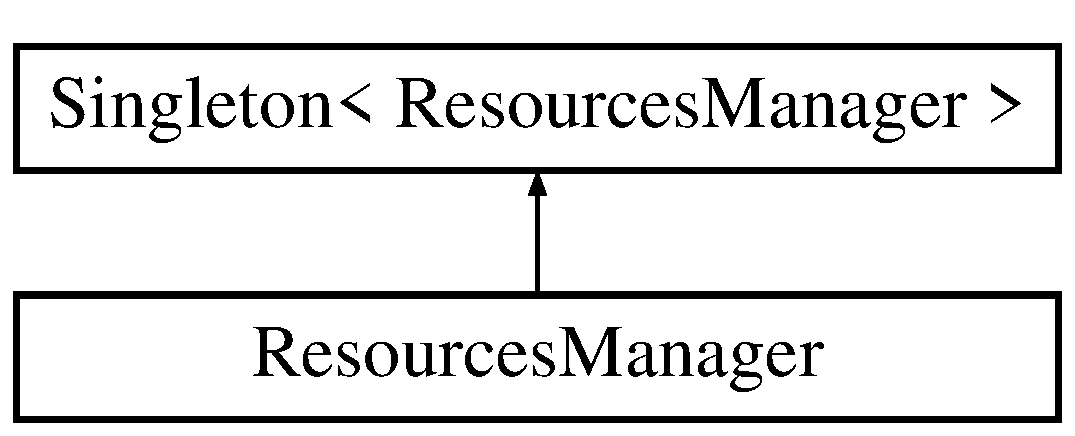
\includegraphics[height=2.000000cm]{class_resources_manager}
\end{center}
\end{figure}
\subsection*{Public Member Functions}
\begin{DoxyCompactItemize}
\item 
\hypertarget{class_resources_manager_abe9a41b9135bf25372c9b31d75c812ee}{\hyperlink{class_shader}{Shader} \& {\bfseries get\+Shader} (const std\+::string \&Name)  throw (std\+::runtime\+\_\+error)}\label{class_resources_manager_abe9a41b9135bf25372c9b31d75c812ee}

\item 
\hypertarget{class_resources_manager_a3e58aed8f31ea5597563535bd26ece09}{{\footnotesize template$<$typename Shader\+Type $>$ }\\Shader\+Type \& {\bfseries get\+Shader} (const std\+::string \&Name)  throw (std\+::runtime\+\_\+error)}\label{class_resources_manager_a3e58aed8f31ea5597563535bd26ece09}

\item 
\hypertarget{class_resources_manager_a2c01ee603157114a93fbfcbbab5e0b0d}{\hyperlink{class_texture}{Texture} \& {\bfseries get\+Texture} (const std\+::string \&Name)  throw (std\+::runtime\+\_\+error)}\label{class_resources_manager_a2c01ee603157114a93fbfcbbab5e0b0d}

\item 
\hypertarget{class_resources_manager_a19915262869d5bcc04fc388c50a7463d}{{\footnotesize template$<$typename T $>$ }\\T \& {\bfseries get\+Texture} (const std\+::string \&Name)  throw (std\+::runtime\+\_\+error)}\label{class_resources_manager_a19915262869d5bcc04fc388c50a7463d}

\item 
\hypertarget{class_resources_manager_a9431bf5993c25da60403f370f77b4317}{\hyperlink{class_program}{Program} \& {\bfseries get\+Program} (const std\+::string \&Name)}\label{class_resources_manager_a9431bf5993c25da60403f370f77b4317}

\item 
\hypertarget{class_resources_manager_a121aa0d53b343fe90e136dc7088ee634}{void {\bfseries reload\+Shaders} ()}\label{class_resources_manager_a121aa0d53b343fe90e136dc7088ee634}

\end{DoxyCompactItemize}
\subsection*{Additional Inherited Members}


The documentation for this class was generated from the following file\+:\begin{DoxyCompactItemize}
\item 
src/\+Core/Resources\+Manager.\+hpp\end{DoxyCompactItemize}

\hypertarget{class_shader}{\section{Shader Class Reference}
\label{class_shader}\index{Shader@{Shader}}
}
Inheritance diagram for Shader\+:\begin{figure}[H]
\begin{center}
\leavevmode
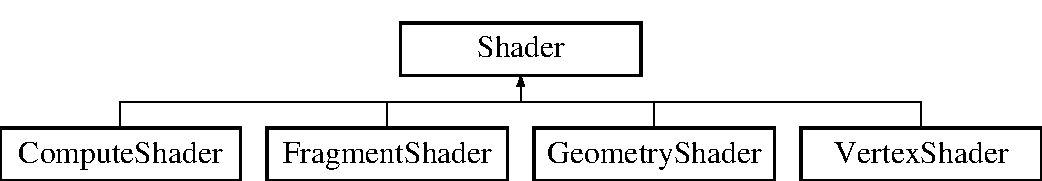
\includegraphics[height=2.000000cm]{class_shader}
\end{center}
\end{figure}
\subsection*{Public Member Functions}
\begin{DoxyCompactItemize}
\item 
\hypertarget{class_shader_a4921f5190ea9a2462b36a14d75b442b3}{void {\bfseries load\+From\+File} (const std\+::string \&path)}\label{class_shader_a4921f5190ea9a2462b36a14d75b442b3}

\item 
\hypertarget{class_shader_a7d3a2d0c4d1dc1c61338459e9ae09d8c}{void {\bfseries reload} ()}\label{class_shader_a7d3a2d0c4d1dc1c61338459e9ae09d8c}

\item 
\hypertarget{class_shader_a2bc90a28b475059544eaaf3054c9bf48}{void {\bfseries set\+Source} (const std\+::string \&src)}\label{class_shader_a2bc90a28b475059544eaaf3054c9bf48}

\item 
\hypertarget{class_shader_a5be69e48ac2436651ead777bf5fb5c9f}{void {\bfseries compile} ()}\label{class_shader_a5be69e48ac2436651ead777bf5fb5c9f}

\item 
\hypertarget{class_shader_a12f70d569014888000fe3da14f0767ac}{const G\+Lint \& {\bfseries get\+I\+D} () const }\label{class_shader_a12f70d569014888000fe3da14f0767ac}

\item 
\hypertarget{class_shader_acd99c9c86c328bfd886541ad508ee21f}{void {\bfseries compute} (G\+Lint x, G\+Lint y=1, G\+Lint z=1)}\label{class_shader_acd99c9c86c328bfd886541ad508ee21f}

\item 
\hypertarget{class_shader_a630c9333e201e7a51a92778c54432022}{bool {\bfseries is\+Valid} () const }\label{class_shader_a630c9333e201e7a51a92778c54432022}

\end{DoxyCompactItemize}
\subsection*{Protected Member Functions}
\begin{DoxyCompactItemize}
\item 
\hypertarget{class_shader_a36de02e8a601c40666bf321f9154577d}{virtual void {\bfseries init\+O\+G\+L} ()=0}\label{class_shader_a36de02e8a601c40666bf321f9154577d}

\end{DoxyCompactItemize}
\subsection*{Protected Attributes}
\begin{DoxyCompactItemize}
\item 
\hypertarget{class_shader_acfef8f5054c8d125f081168b10a38279}{G\+Lint {\bfseries \+\_\+shader} = 0}\label{class_shader_acfef8f5054c8d125f081168b10a38279}

\item 
\hypertarget{class_shader_ac9c918e30c0bb925ab3b39ca3da2db3f}{std\+::string {\bfseries \+\_\+src\+Path} = \char`\"{}\char`\"{}}\label{class_shader_ac9c918e30c0bb925ab3b39ca3da2db3f}

\item 
\hypertarget{class_shader_a0dd6e68a31c1ec8b086a5a6df666823b}{bool {\bfseries \+\_\+compiled} = false}\label{class_shader_a0dd6e68a31c1ec8b086a5a6df666823b}

\end{DoxyCompactItemize}


The documentation for this class was generated from the following files\+:\begin{DoxyCompactItemize}
\item 
src/\+Graphics/\+Shader\+Program/Shader.\+hpp\item 
src/\+Graphics/\+Shader\+Program/Shader.\+cpp\end{DoxyCompactItemize}

\hypertarget{class_singleton}{\section{Singleton$<$ C $>$ Class Template Reference}
\label{class_singleton}\index{Singleton$<$ C $>$@{Singleton$<$ C $>$}}
}


Abstract class for singleton pattern.  




{\ttfamily \#include $<$Singleton.\+hpp$>$}

\subsection*{Static Public Member Functions}
\begin{DoxyCompactItemize}
\item 
static C \& \hyperlink{class_singleton_a3fff22a8380f8ede383d370f2bfb89eb}{get\+Instance} ()
\end{DoxyCompactItemize}
\subsection*{Protected Member Functions}
\begin{DoxyCompactItemize}
\item 
\hypertarget{class_singleton_ae762ebbbd585ece6275ad8e10f5a0938}{{\bfseries Singleton} (const C \&)}\label{class_singleton_ae762ebbbd585ece6275ad8e10f5a0938}

\item 
\hypertarget{class_singleton_a87fd94d3f575a727c898e1f1087fe2a0}{\hyperlink{class_singleton}{Singleton} \& {\bfseries operator=} (const C \&)}\label{class_singleton_a87fd94d3f575a727c898e1f1087fe2a0}

\end{DoxyCompactItemize}


\subsection{Detailed Description}
\subsubsection*{template$<$typename C$>$class Singleton$<$ C $>$}

Abstract class for singleton pattern. 

\subsection{Member Function Documentation}
\hypertarget{class_singleton_a3fff22a8380f8ede383d370f2bfb89eb}{\index{Singleton@{Singleton}!get\+Instance@{get\+Instance}}
\index{get\+Instance@{get\+Instance}!Singleton@{Singleton}}
\subsubsection[{get\+Instance}]{\setlength{\rightskip}{0pt plus 5cm}template$<$typename C$>$ static C\& {\bf Singleton}$<$ C $>$\+::get\+Instance (
\begin{DoxyParamCaption}
{}
\end{DoxyParamCaption}
)\hspace{0.3cm}{\ttfamily [inline]}, {\ttfamily [static]}}}\label{class_singleton_a3fff22a8380f8ede383d370f2bfb89eb}
I think this could be could be set as private without any harm... \begin{DoxyReturn}{Returns}
The instance of C 
\end{DoxyReturn}


The documentation for this class was generated from the following file\+:\begin{DoxyCompactItemize}
\item 
src/\+Tools/Singleton.\+hpp\end{DoxyCompactItemize}

\hypertarget{class_skybox}{\section{Skybox Class Reference}
\label{class_skybox}\index{Skybox@{Skybox}}
}
\subsection*{Public Member Functions}
\begin{DoxyCompactItemize}
\item 
\hypertarget{class_skybox_a8ea7652a84027f1295552ad385da25ab}{{\bfseries Skybox} (const std\+::array$<$ std\+::string, 6 $>$ \&Paths)}\label{class_skybox_a8ea7652a84027f1295552ad385da25ab}

\item 
\hypertarget{class_skybox_ae1df0e8250a0cef935e1edb108329bf7}{void {\bfseries draw} ()}\label{class_skybox_ae1df0e8250a0cef935e1edb108329bf7}

\item 
\hypertarget{class_skybox_a192779bc571cd5079850d7fcd36cbad1}{void {\bfseries load\+Cube\+Map} (const std\+::array$<$ std\+::string, 6 $>$ \&Paths)}\label{class_skybox_a192779bc571cd5079850d7fcd36cbad1}

\item 
\hypertarget{class_skybox_a589d97b0c8fb184b58277b1abcb29c71}{\hyperlink{class_cube_map}{Cube\+Map} \& {\bfseries get\+Cubemap} ()}\label{class_skybox_a589d97b0c8fb184b58277b1abcb29c71}

\end{DoxyCompactItemize}


The documentation for this class was generated from the following files\+:\begin{DoxyCompactItemize}
\item 
src/\+Graphics/Skybox.\+hpp\item 
src/\+Graphics/Skybox.\+cpp\end{DoxyCompactItemize}

\hypertarget{structstbi}{\section{stbi Struct Reference}
\label{structstbi}\index{stbi@{stbi}}
}
\subsection*{Public Attributes}
\begin{DoxyCompactItemize}
\item 
\hypertarget{structstbi_af3b42c257fb0d8896f29ca3921540a42}{uint32 {\bfseries img\+\_\+x}}\label{structstbi_af3b42c257fb0d8896f29ca3921540a42}

\item 
\hypertarget{structstbi_a60cb5a630e268b2d12306c6eca246dd1}{uint32 {\bfseries img\+\_\+y}}\label{structstbi_a60cb5a630e268b2d12306c6eca246dd1}

\item 
\hypertarget{structstbi_ae22cfcc23f5ab67bede22942333ecbd7}{int {\bfseries img\+\_\+n}}\label{structstbi_ae22cfcc23f5ab67bede22942333ecbd7}

\item 
\hypertarget{structstbi_a33f6519d8f99b84afbde795dc7a931f2}{int {\bfseries img\+\_\+out\+\_\+n}}\label{structstbi_a33f6519d8f99b84afbde795dc7a931f2}

\item 
\hypertarget{structstbi_a86596e1eb2b0f57a60a18777bd37ff53}{\hyperlink{structstbi__io__callbacks}{stbi\+\_\+io\+\_\+callbacks} {\bfseries io}}\label{structstbi_a86596e1eb2b0f57a60a18777bd37ff53}

\item 
\hypertarget{structstbi_a9838a0c89630f283c25a16f4e30f40aa}{void $\ast$ {\bfseries io\+\_\+user\+\_\+data}}\label{structstbi_a9838a0c89630f283c25a16f4e30f40aa}

\item 
\hypertarget{structstbi_acb201cc1b3eb134f342cee89f5d11e70}{int {\bfseries read\+\_\+from\+\_\+callbacks}}\label{structstbi_acb201cc1b3eb134f342cee89f5d11e70}

\item 
\hypertarget{structstbi_a76d6f761529ecff7f02469b19371af0e}{int {\bfseries buflen}}\label{structstbi_a76d6f761529ecff7f02469b19371af0e}

\item 
\hypertarget{structstbi_af99edda496281a6ca1b58271cabdbc69}{uint8 {\bfseries buffer\+\_\+start} \mbox{[}128\mbox{]}}\label{structstbi_af99edda496281a6ca1b58271cabdbc69}

\item 
\hypertarget{structstbi_aace36d5487a596bea5faa0aef0398ac8}{uint8 $\ast$ {\bfseries img\+\_\+buffer}}\label{structstbi_aace36d5487a596bea5faa0aef0398ac8}

\item 
\hypertarget{structstbi_a55f78565e605f1784d47fc9acea475f3}{uint8 $\ast$ {\bfseries img\+\_\+buffer\+\_\+end}}\label{structstbi_a55f78565e605f1784d47fc9acea475f3}

\item 
\hypertarget{structstbi_a261be6edda817862e623972b21b4f965}{uint8 $\ast$ {\bfseries img\+\_\+buffer\+\_\+original}}\label{structstbi_a261be6edda817862e623972b21b4f965}

\end{DoxyCompactItemize}


The documentation for this struct was generated from the following file\+:\begin{DoxyCompactItemize}
\item 
src/\+Graphics/stb\+\_\+image.\+cpp\end{DoxyCompactItemize}

\hypertarget{structstbi__gif__lzw__struct}{\section{stbi\+\_\+gif\+\_\+lzw\+\_\+struct Struct Reference}
\label{structstbi__gif__lzw__struct}\index{stbi\+\_\+gif\+\_\+lzw\+\_\+struct@{stbi\+\_\+gif\+\_\+lzw\+\_\+struct}}
}
\subsection*{Public Attributes}
\begin{DoxyCompactItemize}
\item 
\hypertarget{structstbi__gif__lzw__struct_a0e5142cb4117b905eb9efd73c436525c}{int16 {\bfseries prefix}}\label{structstbi__gif__lzw__struct_a0e5142cb4117b905eb9efd73c436525c}

\item 
\hypertarget{structstbi__gif__lzw__struct_a08129c445d56c0983285d6e0e71b83bd}{uint8 {\bfseries first}}\label{structstbi__gif__lzw__struct_a08129c445d56c0983285d6e0e71b83bd}

\item 
\hypertarget{structstbi__gif__lzw__struct_a3ec7f462268018489345b79b2f123764}{uint8 {\bfseries suffix}}\label{structstbi__gif__lzw__struct_a3ec7f462268018489345b79b2f123764}

\end{DoxyCompactItemize}


The documentation for this struct was generated from the following file\+:\begin{DoxyCompactItemize}
\item 
src/\+Graphics/stb\+\_\+image.\+cpp\end{DoxyCompactItemize}

\hypertarget{structstbi__gif__struct}{\section{stbi\+\_\+gif\+\_\+struct Struct Reference}
\label{structstbi__gif__struct}\index{stbi\+\_\+gif\+\_\+struct@{stbi\+\_\+gif\+\_\+struct}}
}
\subsection*{Public Attributes}
\begin{DoxyCompactItemize}
\item 
\hypertarget{structstbi__gif__struct_a28e5c2fb704a64d23a7e8f9013ecda34}{int {\bfseries w}}\label{structstbi__gif__struct_a28e5c2fb704a64d23a7e8f9013ecda34}

\item 
\hypertarget{structstbi__gif__struct_a6ce6b990464cdbbe9a408fe26581b296}{int {\bfseries h}}\label{structstbi__gif__struct_a6ce6b990464cdbbe9a408fe26581b296}

\item 
\hypertarget{structstbi__gif__struct_a1c2d18ea92a86a416e7458cdaa9f4cc3}{stbi\+\_\+uc $\ast$ {\bfseries out}}\label{structstbi__gif__struct_a1c2d18ea92a86a416e7458cdaa9f4cc3}

\item 
\hypertarget{structstbi__gif__struct_a3d22eaa3fe69a1d35ff914add9bb6df5}{int {\bfseries flags}}\label{structstbi__gif__struct_a3d22eaa3fe69a1d35ff914add9bb6df5}

\item 
\hypertarget{structstbi__gif__struct_a0d3690bdbbf0b772d5369c0a29b77cc1}{int {\bfseries bgindex}}\label{structstbi__gif__struct_a0d3690bdbbf0b772d5369c0a29b77cc1}

\item 
\hypertarget{structstbi__gif__struct_ac082648ce87130679bcde2dd4651c530}{int {\bfseries ratio}}\label{structstbi__gif__struct_ac082648ce87130679bcde2dd4651c530}

\item 
\hypertarget{structstbi__gif__struct_ab46e0fb6ad50c3caeac8800ef07b78a8}{int {\bfseries transparent}}\label{structstbi__gif__struct_ab46e0fb6ad50c3caeac8800ef07b78a8}

\item 
\hypertarget{structstbi__gif__struct_aad9790350cb2d775722dc5d55fdfde42}{int {\bfseries eflags}}\label{structstbi__gif__struct_aad9790350cb2d775722dc5d55fdfde42}

\item 
\hypertarget{structstbi__gif__struct_a3d96c452c7935b3a1ca49cc1ce410686}{uint8 {\bfseries pal} \mbox{[}256\mbox{]}\mbox{[}4\mbox{]}}\label{structstbi__gif__struct_a3d96c452c7935b3a1ca49cc1ce410686}

\item 
\hypertarget{structstbi__gif__struct_af2bf4a7890065ce54b8b59c6fd008e5f}{uint8 {\bfseries lpal} \mbox{[}256\mbox{]}\mbox{[}4\mbox{]}}\label{structstbi__gif__struct_af2bf4a7890065ce54b8b59c6fd008e5f}

\item 
\hypertarget{structstbi__gif__struct_a4644d2fe2c84e410ab235ea415e9a740}{\hyperlink{structstbi__gif__lzw__struct}{stbi\+\_\+gif\+\_\+lzw} {\bfseries codes} \mbox{[}4096\mbox{]}}\label{structstbi__gif__struct_a4644d2fe2c84e410ab235ea415e9a740}

\item 
\hypertarget{structstbi__gif__struct_aa10fee29a36ac4b9cae98300f839d091}{uint8 $\ast$ {\bfseries color\+\_\+table}}\label{structstbi__gif__struct_aa10fee29a36ac4b9cae98300f839d091}

\item 
\hypertarget{structstbi__gif__struct_a7a57ec19955875d52af26851ef332db8}{int {\bfseries parse}}\label{structstbi__gif__struct_a7a57ec19955875d52af26851ef332db8}

\item 
\hypertarget{structstbi__gif__struct_a61556e0a3ff8f19fa80401de5da1f079}{int {\bfseries step}}\label{structstbi__gif__struct_a61556e0a3ff8f19fa80401de5da1f079}

\item 
\hypertarget{structstbi__gif__struct_a01e6981357bbd283177f70f87050a49d}{int {\bfseries lflags}}\label{structstbi__gif__struct_a01e6981357bbd283177f70f87050a49d}

\item 
\hypertarget{structstbi__gif__struct_ad3899ad3323686e963a7322e9a80bb05}{int {\bfseries start\+\_\+x}}\label{structstbi__gif__struct_ad3899ad3323686e963a7322e9a80bb05}

\item 
\hypertarget{structstbi__gif__struct_a7f4974b80d6e6f4f56b5fd02a9c1c121}{int {\bfseries start\+\_\+y}}\label{structstbi__gif__struct_a7f4974b80d6e6f4f56b5fd02a9c1c121}

\item 
\hypertarget{structstbi__gif__struct_a02391438194b161d16bdf95878be6a66}{int {\bfseries max\+\_\+x}}\label{structstbi__gif__struct_a02391438194b161d16bdf95878be6a66}

\item 
\hypertarget{structstbi__gif__struct_aff3410e0fff097d4719e54096f6da69b}{int {\bfseries max\+\_\+y}}\label{structstbi__gif__struct_aff3410e0fff097d4719e54096f6da69b}

\item 
\hypertarget{structstbi__gif__struct_adbc7ae7e9ff2e2abdf66eb0e1a4b3ffb}{int {\bfseries cur\+\_\+x}}\label{structstbi__gif__struct_adbc7ae7e9ff2e2abdf66eb0e1a4b3ffb}

\item 
\hypertarget{structstbi__gif__struct_ac61865216c4b578c235f5b8170c2036c}{int {\bfseries cur\+\_\+y}}\label{structstbi__gif__struct_ac61865216c4b578c235f5b8170c2036c}

\item 
\hypertarget{structstbi__gif__struct_a5b7d7625c253025ff5ee4169afbf06b7}{int {\bfseries line\+\_\+size}}\label{structstbi__gif__struct_a5b7d7625c253025ff5ee4169afbf06b7}

\end{DoxyCompactItemize}


The documentation for this struct was generated from the following file\+:\begin{DoxyCompactItemize}
\item 
src/\+Graphics/stb\+\_\+image.\+cpp\end{DoxyCompactItemize}

\hypertarget{structstbi__io__callbacks}{\section{stbi\+\_\+io\+\_\+callbacks Struct Reference}
\label{structstbi__io__callbacks}\index{stbi\+\_\+io\+\_\+callbacks@{stbi\+\_\+io\+\_\+callbacks}}
}
\subsection*{Public Attributes}
\begin{DoxyCompactItemize}
\item 
\hypertarget{structstbi__io__callbacks_a73818f0a4f467e5abfefb1d635f62d82}{int($\ast$ {\bfseries read} )(void $\ast$user, char $\ast$data, int size)}\label{structstbi__io__callbacks_a73818f0a4f467e5abfefb1d635f62d82}

\item 
\hypertarget{structstbi__io__callbacks_afe8270ea04f0c16cdb63f378469df356}{void($\ast$ {\bfseries skip} )(void $\ast$user, unsigned n)}\label{structstbi__io__callbacks_afe8270ea04f0c16cdb63f378469df356}

\item 
\hypertarget{structstbi__io__callbacks_a2c4f3c3b7c75a2e74a35caf74fb8d177}{int($\ast$ {\bfseries eof} )(void $\ast$user)}\label{structstbi__io__callbacks_a2c4f3c3b7c75a2e74a35caf74fb8d177}

\end{DoxyCompactItemize}


The documentation for this struct was generated from the following file\+:\begin{DoxyCompactItemize}
\item 
src/\+Graphics/stb\+\_\+image.\+cpp\end{DoxyCompactItemize}

\hypertarget{structstbi__resample}{\section{stbi\+\_\+resample Struct Reference}
\label{structstbi__resample}\index{stbi\+\_\+resample@{stbi\+\_\+resample}}
}
\subsection*{Public Attributes}
\begin{DoxyCompactItemize}
\item 
\hypertarget{structstbi__resample_a94091463ebc5933cdaf7a813025b6e19}{resample\+\_\+row\+\_\+func {\bfseries resample}}\label{structstbi__resample_a94091463ebc5933cdaf7a813025b6e19}

\item 
\hypertarget{structstbi__resample_a30c51395efffb663b183d7c64def6db3}{uint8 $\ast$ {\bfseries line0}}\label{structstbi__resample_a30c51395efffb663b183d7c64def6db3}

\item 
\hypertarget{structstbi__resample_ac1165a6da3cf652b951056667f89b1f2}{uint8 $\ast$ {\bfseries line1}}\label{structstbi__resample_ac1165a6da3cf652b951056667f89b1f2}

\item 
\hypertarget{structstbi__resample_a1513390ba0102364169a52ff26d5e0f2}{int {\bfseries hs}}\label{structstbi__resample_a1513390ba0102364169a52ff26d5e0f2}

\item 
\hypertarget{structstbi__resample_a331c717f53239339c0c678f92a7bf4d5}{int {\bfseries vs}}\label{structstbi__resample_a331c717f53239339c0c678f92a7bf4d5}

\item 
\hypertarget{structstbi__resample_a41d43c7b0d6caafbf0dfa8ef064bd2a2}{int {\bfseries w\+\_\+lores}}\label{structstbi__resample_a41d43c7b0d6caafbf0dfa8ef064bd2a2}

\item 
\hypertarget{structstbi__resample_a0c479143447d103e73348c89f8b4ef1c}{int {\bfseries ystep}}\label{structstbi__resample_a0c479143447d103e73348c89f8b4ef1c}

\item 
\hypertarget{structstbi__resample_aa1f1ad33e739f7a38fbad8752f64f983}{int {\bfseries ypos}}\label{structstbi__resample_aa1f1ad33e739f7a38fbad8752f64f983}

\end{DoxyCompactItemize}


The documentation for this struct was generated from the following file\+:\begin{DoxyCompactItemize}
\item 
src/\+Graphics/stb\+\_\+image.\+cpp\end{DoxyCompactItemize}

\hypertarget{class_texture}{\section{Texture Class Reference}
\label{class_texture}\index{Texture@{Texture}}
}
Inheritance diagram for Texture\+:\begin{figure}[H]
\begin{center}
\leavevmode
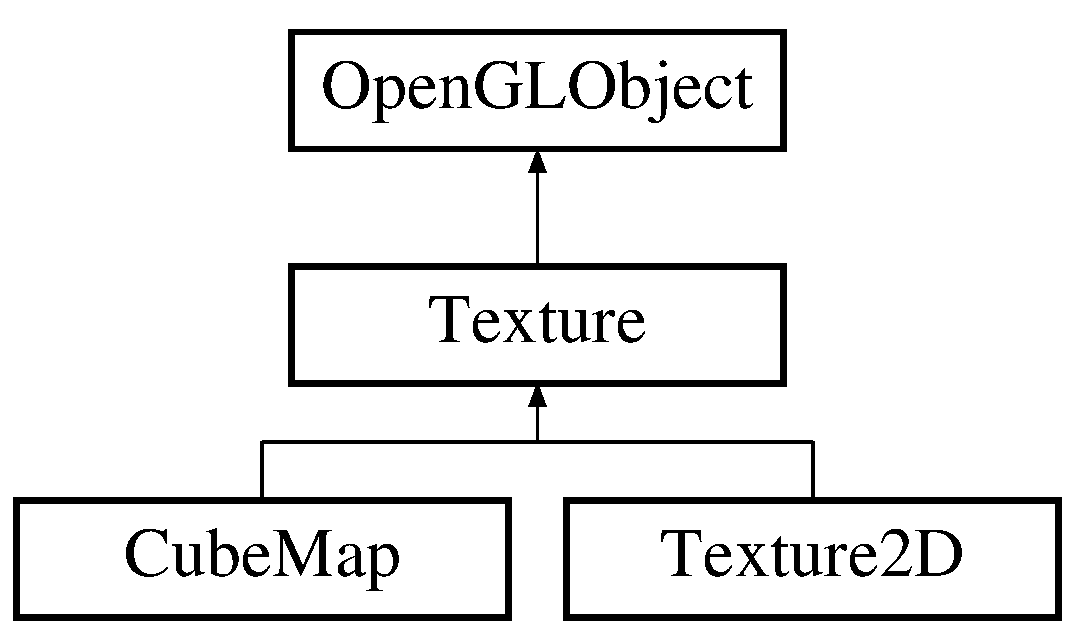
\includegraphics[height=3.000000cm]{class_texture}
\end{center}
\end{figure}
\subsection*{Public Member Functions}
\begin{DoxyCompactItemize}
\item 
\hypertarget{class_texture_ae6e2d1c971338202da0da0e43a48a2d7}{{\bfseries Texture} (G\+Luint handle)}\label{class_texture_ae6e2d1c971338202da0da0e43a48a2d7}

\item 
\hypertarget{class_texture_a045b7ee52dfedc3602549c3706b3b4aa}{{\bfseries Texture} (const \hyperlink{class_texture}{Texture} \&)=default}\label{class_texture_a045b7ee52dfedc3602549c3706b3b4aa}

\item 
\hypertarget{class_texture_a004dd9bd404d90c4be569497aa5540e1}{{\bfseries Texture} (\hyperlink{class_texture}{Texture} \&\&)=default}\label{class_texture_a004dd9bd404d90c4be569497aa5540e1}

\item 
\hypertarget{class_texture_acf93a6e7dd21616a702924ea08faf07d}{\hyperlink{class_texture}{Texture} \& {\bfseries operator=} (const \hyperlink{class_texture}{Texture} \&)=default}\label{class_texture_acf93a6e7dd21616a702924ea08faf07d}

\item 
\hypertarget{class_texture_a612e1d5344d24e0ee9a0ef4a9e876b97}{\hyperlink{class_texture}{Texture} \& {\bfseries operator=} (\hyperlink{class_texture}{Texture} \&\&)=default}\label{class_texture_a612e1d5344d24e0ee9a0ef4a9e876b97}

\item 
\hypertarget{class_texture_a8e5dd00664c3b7ce2d1b402d2cef8b45}{virtual void {\bfseries bind} (int Unit\+Texture=0) const }\label{class_texture_a8e5dd00664c3b7ce2d1b402d2cef8b45}

\end{DoxyCompactItemize}
\subsection*{Protected Member Functions}
\begin{DoxyCompactItemize}
\item 
\hypertarget{class_texture_ae13a97cde8768d3b61fd9524c21fbfac}{void {\bfseries cleanup} ()}\label{class_texture_ae13a97cde8768d3b61fd9524c21fbfac}

\end{DoxyCompactItemize}


The documentation for this class was generated from the following files\+:\begin{DoxyCompactItemize}
\item 
src/\+Graphics/Texture.\+hpp\item 
src/\+Graphics/Texture.\+cpp\end{DoxyCompactItemize}

\hypertarget{class_texture2_d}{\section{Texture2\+D Class Reference}
\label{class_texture2_d}\index{Texture2\+D@{Texture2\+D}}
}
Inheritance diagram for Texture2\+D\+:\begin{figure}[H]
\begin{center}
\leavevmode
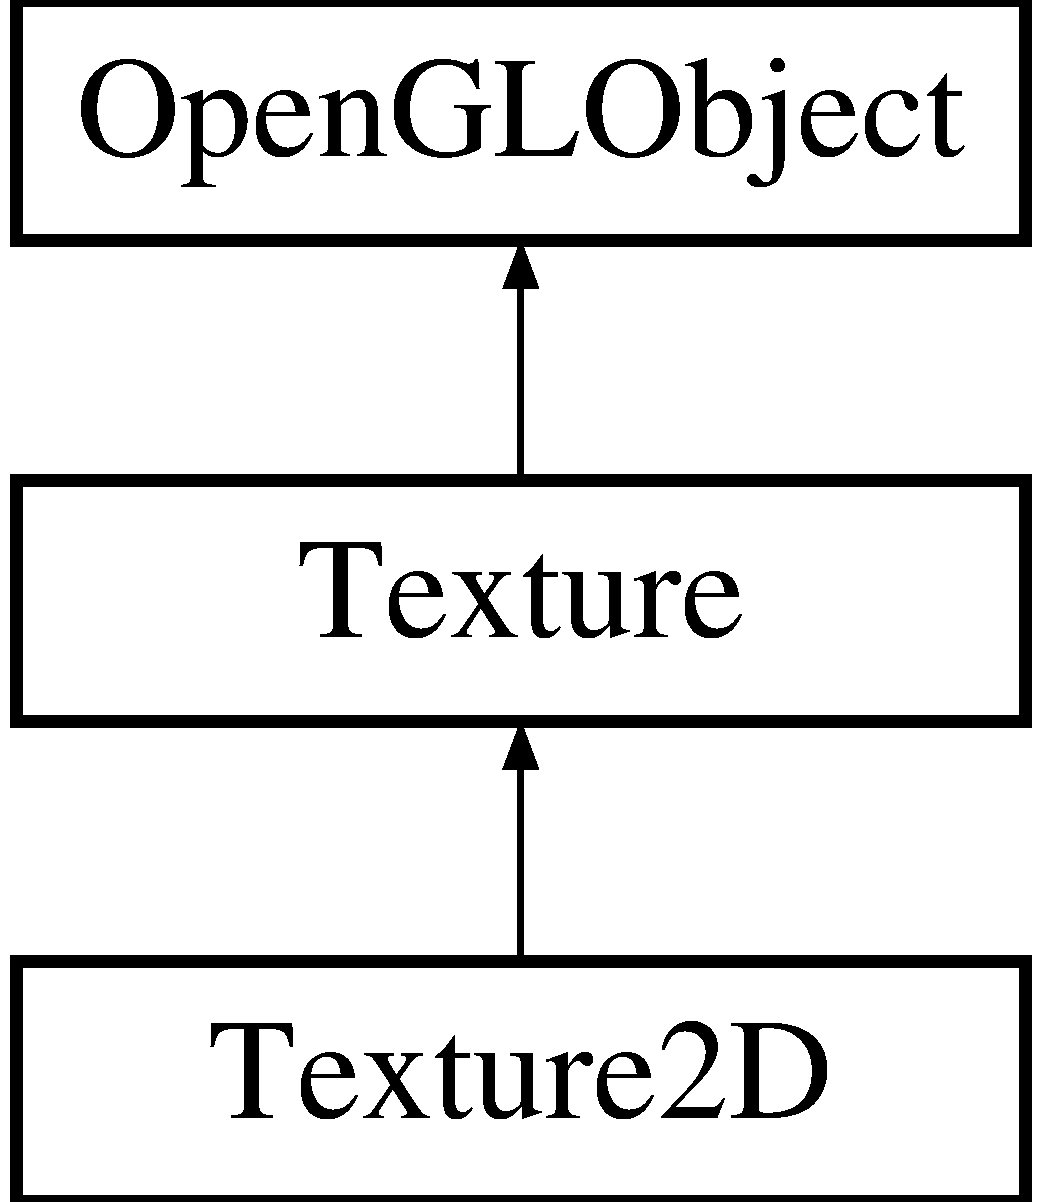
\includegraphics[height=3.000000cm]{class_texture2_d}
\end{center}
\end{figure}
\subsection*{Public Member Functions}
\begin{DoxyCompactItemize}
\item 
\hypertarget{class_texture2_d_a2f34b32ade581a7c2c51d33f073b7d6e}{void {\bfseries load} (const std\+::string \&Path)}\label{class_texture2_d_a2f34b32ade581a7c2c51d33f073b7d6e}

\item 
\hypertarget{class_texture2_d_abb1f4151f215b0c6b320d4655012f43b}{void {\bfseries create} (const void $\ast$data, size\+\_\+t width, size\+\_\+t height, int comp\+Count)}\label{class_texture2_d_abb1f4151f215b0c6b320d4655012f43b}

\item 
\hypertarget{class_texture2_d_a02b088645b5b17bfad6dadc62522df41}{virtual void {\bfseries bind} (int Unit\+Texture=0) const }\label{class_texture2_d_a02b088645b5b17bfad6dadc62522df41}

\end{DoxyCompactItemize}
\subsection*{Static Public Member Functions}
\begin{DoxyCompactItemize}
\item 
\hypertarget{class_texture2_d_ac21f1e200e9aa03d7371614e3026b079}{static void {\bfseries unbind} ()}\label{class_texture2_d_ac21f1e200e9aa03d7371614e3026b079}

\end{DoxyCompactItemize}
\subsection*{Additional Inherited Members}


The documentation for this class was generated from the following files\+:\begin{DoxyCompactItemize}
\item 
src/\+Graphics/Texture2\+D.\+hpp\item 
src/\+Graphics/Texture2\+D.\+cpp\end{DoxyCompactItemize}

\hypertarget{class_time_manager}{\section{Time\+Manager Class Reference}
\label{class_time_manager}\index{Time\+Manager@{Time\+Manager}}
}
Inheritance diagram for Time\+Manager\+:\begin{figure}[H]
\begin{center}
\leavevmode
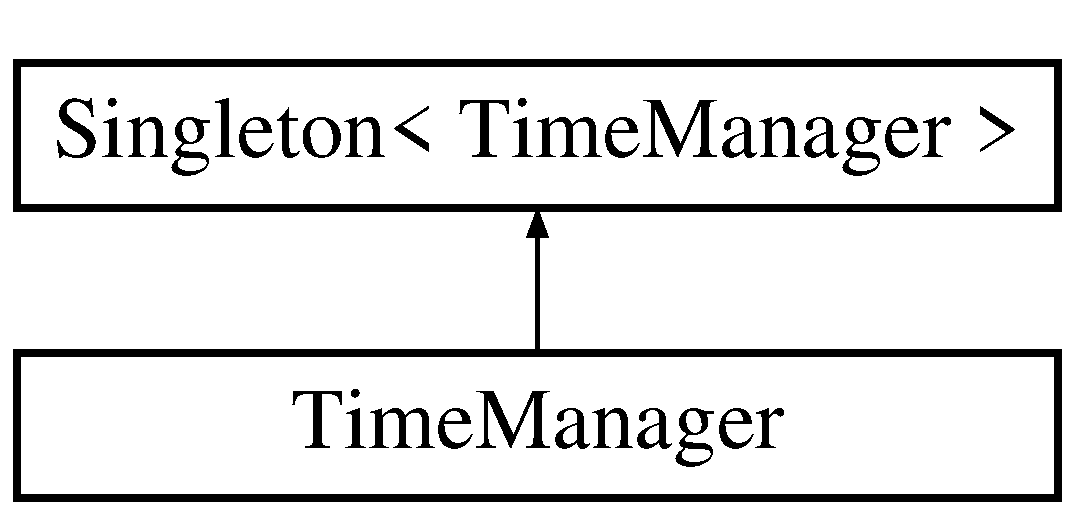
\includegraphics[height=2.000000cm]{class_time_manager}
\end{center}
\end{figure}
\subsection*{Public Types}
\begin{DoxyCompactItemize}
\item 
\hypertarget{class_time_manager_a09f5df0345b8e585badbd57cbaf3b506}{using {\bfseries Real} = double}\label{class_time_manager_a09f5df0345b8e585badbd57cbaf3b506}

\item 
\hypertarget{class_time_manager_a4162b0016503de524079dd23e68ba697}{using {\bfseries Time\+Point} = std\+::chrono\+::high\+\_\+resolution\+\_\+clock\+::time\+\_\+point}\label{class_time_manager_a4162b0016503de524079dd23e68ba697}

\item 
\hypertarget{class_time_manager_a93d275e53c96a786c78b9b31cd729fb3}{using {\bfseries Seconds} = std\+::chrono\+::duration$<$ Real $>$}\label{class_time_manager_a93d275e53c96a786c78b9b31cd729fb3}

\end{DoxyCompactItemize}
\subsection*{Public Member Functions}
\begin{DoxyCompactItemize}
\item 
\hyperlink{class_time_manager_ab1c3cbb48ad68d928bb8b9a4ef210ed6}{Time\+Manager} ()
\begin{DoxyCompactList}\small\item\em Default Constructor. \end{DoxyCompactList}\item 
\hypertarget{class_time_manager_a97d902b19861efc099141eeb846671a3}{void \hyperlink{class_time_manager_a97d902b19861efc099141eeb846671a3}{update} ()}\label{class_time_manager_a97d902b19861efc099141eeb846671a3}

\begin{DoxyCompactList}\small\item\em Manages the internals timers -\/ should be called once each frame. This is where the actual job is done ! \end{DoxyCompactList}\item 
\hypertarget{class_time_manager_ae47f04150537e55eab595762e0bb0d18}{Real \hyperlink{class_time_manager_ae47f04150537e55eab595762e0bb0d18}{get\+Timerate} () const }\label{class_time_manager_ae47f04150537e55eab595762e0bb0d18}

\begin{DoxyCompactList}\small\item\em Returns the current Timerate (1.\+f means normal game speed, always $>$= 0.\+f) \end{DoxyCompactList}\item 
void \hyperlink{class_time_manager_a59b542c461ec5142fecd03b78e105fcd}{set\+Timerate} (Real value)
\begin{DoxyCompactList}\small\item\em Sets the timerate to value. \end{DoxyCompactList}\item 
\hypertarget{class_time_manager_aa65b353c86f1c628a904888fd5ff0cf2}{Real \hyperlink{class_time_manager_aa65b353c86f1c628a904888fd5ff0cf2}{get\+Real\+Delta\+Time} () const }\label{class_time_manager_aa65b353c86f1c628a904888fd5ff0cf2}

\begin{DoxyCompactList}\small\item\em Returns the last frame 'real' time duration in seconds This is clamped to avoid 0 cancelation at really high F\+P\+S and too long frames (when moving the window for example). \end{DoxyCompactList}\item 
\hypertarget{class_time_manager_ae9f23854e9a4bc1af43cb528acfbdf8e}{Real \hyperlink{class_time_manager_ae9f23854e9a4bc1af43cb528acfbdf8e}{get\+Delta\+Time} () const }\label{class_time_manager_ae9f23854e9a4bc1af43cb528acfbdf8e}

\begin{DoxyCompactList}\small\item\em Returns the last frame in-\/game duration in seconds (equivalent to \hyperlink{class_time_manager_ae47f04150537e55eab595762e0bb0d18}{get\+Timerate()}$\ast$get\+Real\+Delta\+Time()) \end{DoxyCompactList}\item 
\hypertarget{class_time_manager_a6d952d8906d03dce397c7e2835adad1b}{Real \hyperlink{class_time_manager_a6d952d8906d03dce397c7e2835adad1b}{get\+Instant\+Frame\+Rate} () const }\label{class_time_manager_a6d952d8906d03dce397c7e2835adad1b}

\begin{DoxyCompactList}\small\item\em Returns frame rate based on the last frame duration. \end{DoxyCompactList}\item 
\hypertarget{class_time_manager_a8941e2d56292730e3301d0920da7e658}{Real {\bfseries get\+Runtime} () const }\label{class_time_manager_a8941e2d56292730e3301d0920da7e658}

\item 
\hypertarget{class_time_manager_a3c48c5df2a7dcbcf23f8acdd5872705c}{float \& {\bfseries get\+Runtime\+Ref} ()}\label{class_time_manager_a3c48c5df2a7dcbcf23f8acdd5872705c}

\end{DoxyCompactItemize}
\subsection*{Additional Inherited Members}


\subsection{Constructor \& Destructor Documentation}
\hypertarget{class_time_manager_ab1c3cbb48ad68d928bb8b9a4ef210ed6}{\index{Time\+Manager@{Time\+Manager}!Time\+Manager@{Time\+Manager}}
\index{Time\+Manager@{Time\+Manager}!Time\+Manager@{Time\+Manager}}
\subsubsection[{Time\+Manager}]{\setlength{\rightskip}{0pt plus 5cm}Time\+Manager\+::\+Time\+Manager (
\begin{DoxyParamCaption}
{}
\end{DoxyParamCaption}
)}}\label{class_time_manager_ab1c3cbb48ad68d928bb8b9a4ef210ed6}


Default Constructor. 



\subsection{Member Function Documentation}
\hypertarget{class_time_manager_a59b542c461ec5142fecd03b78e105fcd}{\index{Time\+Manager@{Time\+Manager}!set\+Timerate@{set\+Timerate}}
\index{set\+Timerate@{set\+Timerate}!Time\+Manager@{Time\+Manager}}
\subsubsection[{set\+Timerate}]{\setlength{\rightskip}{0pt plus 5cm}void Time\+Manager\+::set\+Timerate (
\begin{DoxyParamCaption}
\item[{Real}]{value}
\end{DoxyParamCaption}
)\hspace{0.3cm}{\ttfamily [inline]}}}\label{class_time_manager_a59b542c461ec5142fecd03b78e105fcd}


Sets the timerate to value. 


\begin{DoxyParams}{Parameters}
{\em value} & \\
\hline
\end{DoxyParams}


The documentation for this class was generated from the following files\+:\begin{DoxyCompactItemize}
\item 
src/\+Core/Time\+Manager.\+hpp\item 
src/\+Core/Time\+Manager.\+cpp\end{DoxyCompactItemize}

\hypertarget{class_timer}{\section{Timer Class Reference}
\label{class_timer}\index{Timer@{Timer}}
}


{\ttfamily \#include $<$Timer.\+hpp$>$}

\subsection*{Public Member Functions}
\begin{DoxyCompactItemize}
\item 
\hyperlink{class_timer_aab51589602494ed3f9aba851dc00ff45}{Timer} (bool run=false)
\item 
\hypertarget{class_timer_a3a8b5272198d029779dc9302a54305a8}{void {\bfseries start} ()}\label{class_timer_a3a8b5272198d029779dc9302a54305a8}

\item 
\hypertarget{class_timer_a9020542d73357a4eef512eefaf57524b}{void {\bfseries reset} ()}\label{class_timer_a9020542d73357a4eef512eefaf57524b}

\item 
\hypertarget{class_timer_a0289effad7b573c508bc27e405900a23}{void {\bfseries pause} ()}\label{class_timer_a0289effad7b573c508bc27e405900a23}

\item 
\hypertarget{class_timer_aa4dd50d7ed48ac73efed2950749d35d6}{void {\bfseries unpause} ()}\label{class_timer_aa4dd50d7ed48ac73efed2950749d35d6}

\item 
{\footnotesize template$<$typename Unit $>$ }\\Unit \hyperlink{class_timer_a36b9bf710c37b6394c93960c515ba20c}{running\+Time} () const 
\item 
std\+::chrono\+::nanoseconds \hyperlink{class_timer_a9c9acd2b0e51984bbaf6b066f0b47f03}{nanoseconds} () const 
\item 
std\+::chrono\+::microseconds \hyperlink{class_timer_a9965655cf9bd4ee646af97e7558797e3}{microseconds} () const 
\item 
std\+::chrono\+::milliseconds \hyperlink{class_timer_a39c96e027b87ce416be309668dc02c2a}{milliseconds} () const 
\item 
std\+::chrono\+::seconds \hyperlink{class_timer_a9eea487e771e45f9983e4cb8aab3f876}{seconds} () const 
\end{DoxyCompactItemize}
\subsection*{Friends}
\begin{DoxyCompactItemize}
\item 
\hypertarget{class_timer_abbdf0c13bc0413398fc244c28299f5b4}{{\footnotesize template$<$typename Char\+T , typename Traits $>$ }\\std\+::basic\+\_\+ostream$<$ Char\+T, \\*
Traits $>$ \& {\bfseries operator$<$$<$} (std\+::basic\+\_\+ostream$<$ Char\+T, Traits $>$ \&out, const \hyperlink{class_timer}{Timer} \&t)}\label{class_timer_abbdf0c13bc0413398fc244c28299f5b4}

\end{DoxyCompactItemize}


\subsection{Detailed Description}
Extremely simple \hyperlink{class_timer}{Timer} class using C++11 chrono library 

\subsection{Constructor \& Destructor Documentation}
\hypertarget{class_timer_aab51589602494ed3f9aba851dc00ff45}{\index{Timer@{Timer}!Timer@{Timer}}
\index{Timer@{Timer}!Timer@{Timer}}
\subsubsection[{Timer}]{\setlength{\rightskip}{0pt plus 5cm}Timer\+::\+Timer (
\begin{DoxyParamCaption}
\item[{bool}]{run = {\ttfamily false}}
\end{DoxyParamCaption}
)\hspace{0.3cm}{\ttfamily [inline]}, {\ttfamily [explicit]}}}\label{class_timer_aab51589602494ed3f9aba851dc00ff45}

\begin{DoxyParams}{Parameters}
{\em run} & Pass true to start the \hyperlink{class_timer}{Timer} right away \\
\hline
\end{DoxyParams}


\subsection{Member Function Documentation}
\hypertarget{class_timer_a9965655cf9bd4ee646af97e7558797e3}{\index{Timer@{Timer}!microseconds@{microseconds}}
\index{microseconds@{microseconds}!Timer@{Timer}}
\subsubsection[{microseconds}]{\setlength{\rightskip}{0pt plus 5cm}std\+::chrono\+::microseconds Timer\+::microseconds (
\begin{DoxyParamCaption}
{}
\end{DoxyParamCaption}
) const\hspace{0.3cm}{\ttfamily [inline]}}}\label{class_timer_a9965655cf9bd4ee646af97e7558797e3}
\begin{DoxyReturn}{Returns}
Running time in microseconds 
\end{DoxyReturn}
\hypertarget{class_timer_a39c96e027b87ce416be309668dc02c2a}{\index{Timer@{Timer}!milliseconds@{milliseconds}}
\index{milliseconds@{milliseconds}!Timer@{Timer}}
\subsubsection[{milliseconds}]{\setlength{\rightskip}{0pt plus 5cm}std\+::chrono\+::milliseconds Timer\+::milliseconds (
\begin{DoxyParamCaption}
{}
\end{DoxyParamCaption}
) const\hspace{0.3cm}{\ttfamily [inline]}}}\label{class_timer_a39c96e027b87ce416be309668dc02c2a}
\begin{DoxyReturn}{Returns}
Running time in milliseconds 
\end{DoxyReturn}
\hypertarget{class_timer_a9c9acd2b0e51984bbaf6b066f0b47f03}{\index{Timer@{Timer}!nanoseconds@{nanoseconds}}
\index{nanoseconds@{nanoseconds}!Timer@{Timer}}
\subsubsection[{nanoseconds}]{\setlength{\rightskip}{0pt plus 5cm}std\+::chrono\+::nanoseconds Timer\+::nanoseconds (
\begin{DoxyParamCaption}
{}
\end{DoxyParamCaption}
) const\hspace{0.3cm}{\ttfamily [inline]}}}\label{class_timer_a9c9acd2b0e51984bbaf6b066f0b47f03}
\begin{DoxyReturn}{Returns}
Running time in nanoseconds 
\end{DoxyReturn}
\hypertarget{class_timer_a36b9bf710c37b6394c93960c515ba20c}{\index{Timer@{Timer}!running\+Time@{running\+Time}}
\index{running\+Time@{running\+Time}!Timer@{Timer}}
\subsubsection[{running\+Time}]{\setlength{\rightskip}{0pt plus 5cm}template$<$typename Unit $>$ Unit Timer\+::running\+Time (
\begin{DoxyParamCaption}
{}
\end{DoxyParamCaption}
) const\hspace{0.3cm}{\ttfamily [inline]}}}\label{class_timer_a36b9bf710c37b6394c93960c515ba20c}
\begin{DoxyReturn}{Returns}
Running time in Unit 
\end{DoxyReturn}
\hypertarget{class_timer_a9eea487e771e45f9983e4cb8aab3f876}{\index{Timer@{Timer}!seconds@{seconds}}
\index{seconds@{seconds}!Timer@{Timer}}
\subsubsection[{seconds}]{\setlength{\rightskip}{0pt plus 5cm}std\+::chrono\+::seconds Timer\+::seconds (
\begin{DoxyParamCaption}
{}
\end{DoxyParamCaption}
) const\hspace{0.3cm}{\ttfamily [inline]}}}\label{class_timer_a9eea487e771e45f9983e4cb8aab3f876}
\begin{DoxyReturn}{Returns}
Running time in seconds 
\end{DoxyReturn}


The documentation for this class was generated from the following file\+:\begin{DoxyCompactItemize}
\item 
src/Timer.\+hpp\end{DoxyCompactItemize}

\hypertarget{class_uniform}{\section{Uniform$<$ T $>$ Class Template Reference}
\label{class_uniform}\index{Uniform$<$ T $>$@{Uniform$<$ T $>$}}
}
Inheritance diagram for Uniform$<$ T $>$\+:\begin{figure}[H]
\begin{center}
\leavevmode
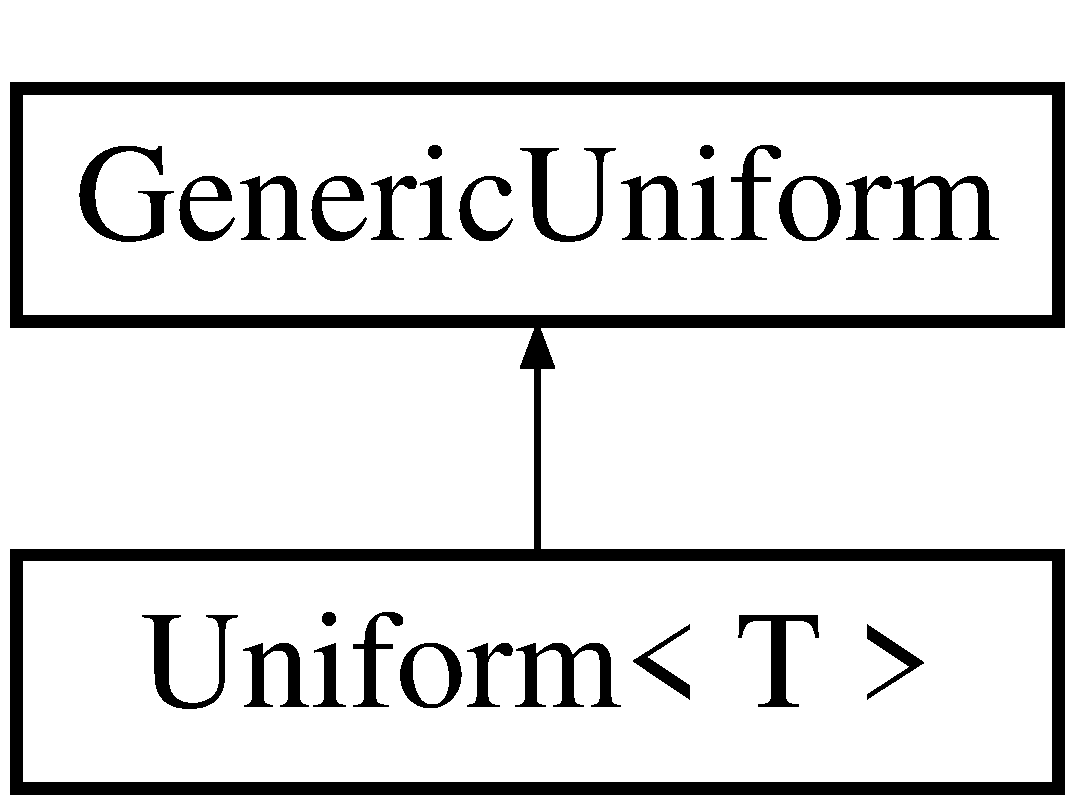
\includegraphics[height=2.000000cm]{class_uniform}
\end{center}
\end{figure}
\subsection*{Public Member Functions}
\begin{DoxyCompactItemize}
\item 
\hypertarget{class_uniform_af7f95b778e5625ce1416208a18ee1b47}{{\bfseries Uniform} (const std\+::string \&N, G\+Luint L, T \&V)}\label{class_uniform_af7f95b778e5625ce1416208a18ee1b47}

\item 
\hypertarget{class_uniform_a52faf85388dfdf7e093fe9c50552309a}{const T \& {\bfseries get\+Value} () const }\label{class_uniform_a52faf85388dfdf7e093fe9c50552309a}

\item 
\hypertarget{class_uniform_a1965859a7d6949b9b93bd04228986506}{T \& {\bfseries get\+Ref\+To\+Value} ()}\label{class_uniform_a1965859a7d6949b9b93bd04228986506}

\item 
\hypertarget{class_uniform_aaf1506224a2db50568592d2d1ba69903}{void {\bfseries set\+Value} (const T \&val)}\label{class_uniform_aaf1506224a2db50568592d2d1ba69903}

\end{DoxyCompactItemize}


The documentation for this class was generated from the following file\+:\begin{DoxyCompactItemize}
\item 
src/\+Graphics/\+Shader\+Program/\+W\+I\+P/Uniform.\+hpp\end{DoxyCompactItemize}

\hypertarget{class_material_1_1_uniform}{\section{Material\+:\+:Uniform$<$ T $>$ Class Template Reference}
\label{class_material_1_1_uniform}\index{Material\+::\+Uniform$<$ T $>$@{Material\+::\+Uniform$<$ T $>$}}
}
\subsection*{Public Member Functions}
\begin{DoxyCompactItemize}
\item 
\hypertarget{class_material_1_1_uniform_a6912f28ba6af514c004e35eb9d6ea9ac}{{\bfseries Uniform} (const std\+::string \&N, G\+Luint L, T \&V)}\label{class_material_1_1_uniform_a6912f28ba6af514c004e35eb9d6ea9ac}

\item 
\hypertarget{class_material_1_1_uniform_a903bf4b04b191c5e543de6b0b10d03e9}{const std\+::string \& {\bfseries get\+Name} () const }\label{class_material_1_1_uniform_a903bf4b04b191c5e543de6b0b10d03e9}

\item 
\hypertarget{class_material_1_1_uniform_ab574c10af2d35fecb57a80c15b874168}{G\+Luint {\bfseries get\+Location} () const }\label{class_material_1_1_uniform_ab574c10af2d35fecb57a80c15b874168}

\item 
\hypertarget{class_material_1_1_uniform_ac7387f4672029743feb6ff0cf6446d93}{const T \& {\bfseries get\+Value} () const }\label{class_material_1_1_uniform_ac7387f4672029743feb6ff0cf6446d93}

\item 
\hypertarget{class_material_1_1_uniform_a3fa5fa36c8804f508868ef6a7a300bc8}{T \& {\bfseries get\+Ref\+To\+Value} ()}\label{class_material_1_1_uniform_a3fa5fa36c8804f508868ef6a7a300bc8}

\item 
\hypertarget{class_material_1_1_uniform_ab28ca1784fbe6386966298b257150987}{void {\bfseries set\+Value} (const T \&val)}\label{class_material_1_1_uniform_ab28ca1784fbe6386966298b257150987}

\item 
\hypertarget{class_material_1_1_uniform_a5d61dff1eeb82a8c4b962ce2af0a1c8f}{void {\bfseries set\+Location} (const G\+Luint val)}\label{class_material_1_1_uniform_a5d61dff1eeb82a8c4b962ce2af0a1c8f}

\end{DoxyCompactItemize}


The documentation for this class was generated from the following file\+:\begin{DoxyCompactItemize}
\item 
src/\+Graphics/Material.\+hpp\end{DoxyCompactItemize}

\hypertarget{class_uniform_3_01_texture_01_4}{\section{Uniform$<$ Texture $>$ Class Template Reference}
\label{class_uniform_3_01_texture_01_4}\index{Uniform$<$ Texture $>$@{Uniform$<$ Texture $>$}}
}
Inheritance diagram for Uniform$<$ Texture $>$\+:\begin{figure}[H]
\begin{center}
\leavevmode
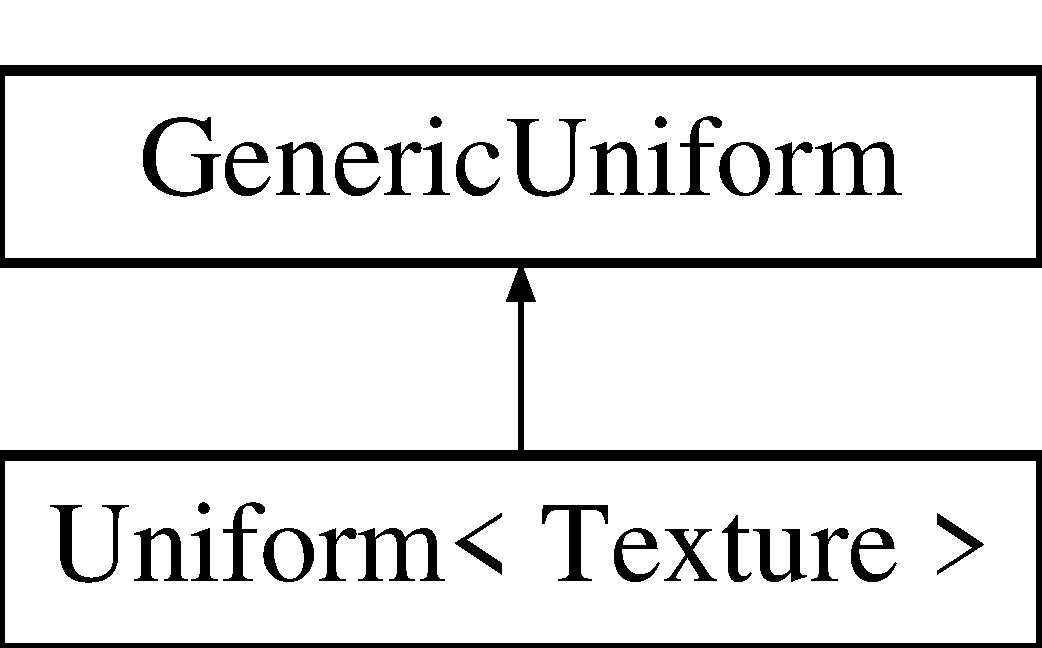
\includegraphics[height=2.000000cm]{class_uniform_3_01_texture_01_4}
\end{center}
\end{figure}
\subsection*{Public Member Functions}
\begin{DoxyCompactItemize}
\item 
\hypertarget{class_uniform_3_01_texture_01_4_a56e03be30efbb0beb0fd356343741ee3}{{\bfseries Uniform} (const std\+::string \&N, G\+Luint L, G\+Luint U, \hyperlink{class_texture}{Texture} \&V)}\label{class_uniform_3_01_texture_01_4_a56e03be30efbb0beb0fd356343741ee3}

\item 
\hypertarget{class_uniform_3_01_texture_01_4_a7e1cb5a42c1766e602ef25d1b6bcb7cf}{const \hyperlink{class_texture}{Texture} \& {\bfseries get\+Value} () const }\label{class_uniform_3_01_texture_01_4_a7e1cb5a42c1766e602ef25d1b6bcb7cf}

\item 
\hypertarget{class_uniform_3_01_texture_01_4_a07a88dbb88bc7a44f21cf4f1bde32193}{\hyperlink{class_texture}{Texture} \& {\bfseries get\+Ref\+To\+Value} ()}\label{class_uniform_3_01_texture_01_4_a07a88dbb88bc7a44f21cf4f1bde32193}

\item 
\hypertarget{class_uniform_3_01_texture_01_4_a43d9c62a0aaca5df68d72dd8c5136eab}{G\+Luint {\bfseries get\+Texture\+Unit} () const }\label{class_uniform_3_01_texture_01_4_a43d9c62a0aaca5df68d72dd8c5136eab}

\item 
\hypertarget{class_uniform_3_01_texture_01_4_af55eb2ce9d0ba8a448ab72ab286ecd8c}{void {\bfseries set\+Value} (const \hyperlink{class_texture}{Texture} \&val)}\label{class_uniform_3_01_texture_01_4_af55eb2ce9d0ba8a448ab72ab286ecd8c}

\item 
\hypertarget{class_uniform_3_01_texture_01_4_a747f5b109a680fe9f8a7ca03618f8200}{void {\bfseries set\+Texture\+Unit} (G\+Luint U)}\label{class_uniform_3_01_texture_01_4_a747f5b109a680fe9f8a7ca03618f8200}

\end{DoxyCompactItemize}


The documentation for this class was generated from the following file\+:\begin{DoxyCompactItemize}
\item 
src/\+Graphics/\+Shader\+Program/\+W\+I\+P/Uniform.\+hpp\end{DoxyCompactItemize}

\hypertarget{class_vertex_shader}{\section{Vertex\+Shader Class Reference}
\label{class_vertex_shader}\index{Vertex\+Shader@{Vertex\+Shader}}
}
Inheritance diagram for Vertex\+Shader\+:\begin{figure}[H]
\begin{center}
\leavevmode
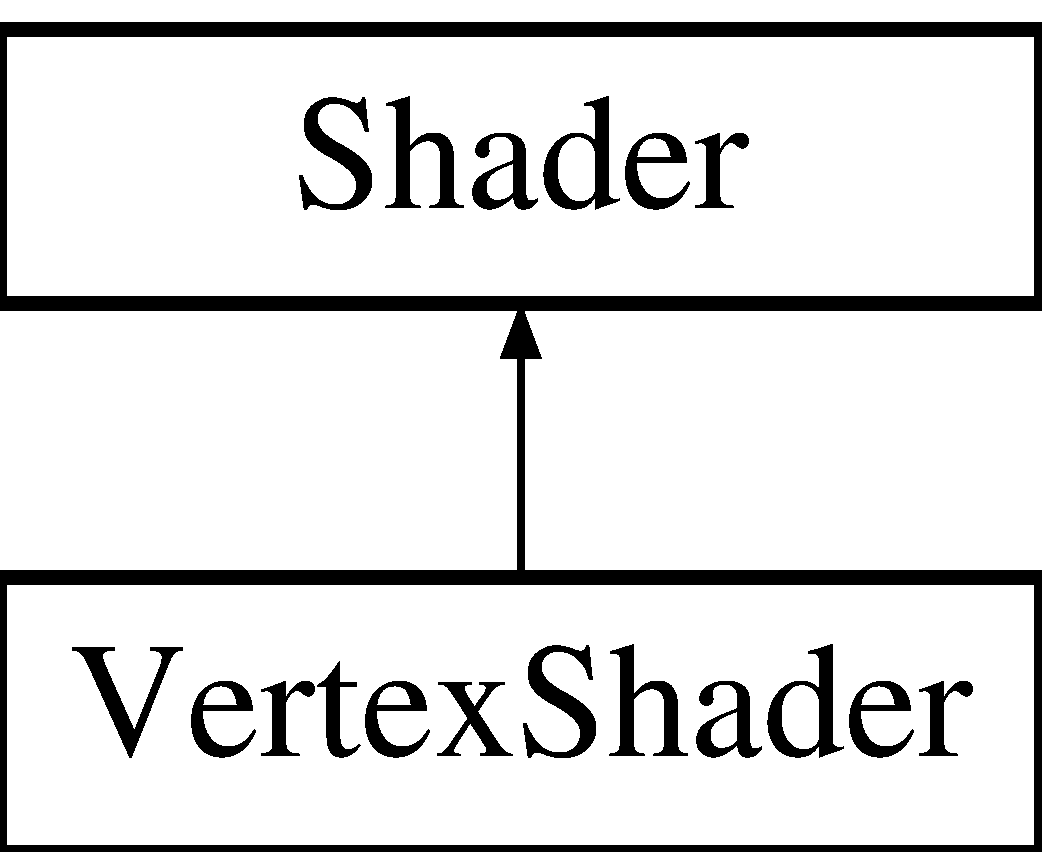
\includegraphics[height=2.000000cm]{class_vertex_shader}
\end{center}
\end{figure}
\subsection*{Additional Inherited Members}


The documentation for this class was generated from the following files\+:\begin{DoxyCompactItemize}
\item 
src/\+Graphics/\+Shader\+Program/Vertex\+Shader.\+hpp\item 
src/\+Graphics/\+Shader\+Program/Vertex\+Shader.\+cpp\end{DoxyCompactItemize}

\hypertarget{structzbuf}{\section{zbuf Struct Reference}
\label{structzbuf}\index{zbuf@{zbuf}}
}
\subsection*{Public Attributes}
\begin{DoxyCompactItemize}
\item 
\hypertarget{structzbuf_a7080eb91dcc67e1dfe818d08e6f22c4e}{uint8 $\ast$ {\bfseries zbuffer}}\label{structzbuf_a7080eb91dcc67e1dfe818d08e6f22c4e}

\item 
\hypertarget{structzbuf_af030baa17bebedd18272678da17a33f4}{uint8 $\ast$ {\bfseries zbuffer\+\_\+end}}\label{structzbuf_af030baa17bebedd18272678da17a33f4}

\item 
\hypertarget{structzbuf_acd069cdb4100884a732ad2794edbbdff}{int {\bfseries num\+\_\+bits}}\label{structzbuf_acd069cdb4100884a732ad2794edbbdff}

\item 
\hypertarget{structzbuf_a3bb8244d7be17801079c5a8587182edb}{uint32 {\bfseries code\+\_\+buffer}}\label{structzbuf_a3bb8244d7be17801079c5a8587182edb}

\item 
\hypertarget{structzbuf_aaf137c25fa5b9fb14e92354da4203c38}{char $\ast$ {\bfseries zout}}\label{structzbuf_aaf137c25fa5b9fb14e92354da4203c38}

\item 
\hypertarget{structzbuf_af31571e8d74c78c9bb18d92205150b28}{char $\ast$ {\bfseries zout\+\_\+start}}\label{structzbuf_af31571e8d74c78c9bb18d92205150b28}

\item 
\hypertarget{structzbuf_af07c0b7b7227f670ee1413bc0dcab791}{char $\ast$ {\bfseries zout\+\_\+end}}\label{structzbuf_af07c0b7b7227f670ee1413bc0dcab791}

\item 
\hypertarget{structzbuf_ae662f24e0973ca19b543e64647a6bfb6}{int {\bfseries z\+\_\+expandable}}\label{structzbuf_ae662f24e0973ca19b543e64647a6bfb6}

\item 
\hypertarget{structzbuf_a5906bdbe9dfb565339acac51af9efe89}{\hyperlink{structzhuffman}{zhuffman} {\bfseries z\+\_\+length}}\label{structzbuf_a5906bdbe9dfb565339acac51af9efe89}

\item 
\hypertarget{structzbuf_ae7d9588b2548708e14f3c6ad89bf26b5}{\hyperlink{structzhuffman}{zhuffman} {\bfseries z\+\_\+distance}}\label{structzbuf_ae7d9588b2548708e14f3c6ad89bf26b5}

\end{DoxyCompactItemize}


The documentation for this struct was generated from the following file\+:\begin{DoxyCompactItemize}
\item 
src/\+Graphics/stb\+\_\+image.\+cpp\end{DoxyCompactItemize}

\hypertarget{structzhuffman}{\section{zhuffman Struct Reference}
\label{structzhuffman}\index{zhuffman@{zhuffman}}
}
\subsection*{Public Attributes}
\begin{DoxyCompactItemize}
\item 
\hypertarget{structzhuffman_a12d5f92a121b65680e5f0b4027d00c96}{uint16 {\bfseries fast} \mbox{[}1$<$$<$ Z\+F\+A\+S\+T\+\_\+\+B\+I\+T\+S\mbox{]}}\label{structzhuffman_a12d5f92a121b65680e5f0b4027d00c96}

\item 
\hypertarget{structzhuffman_a81f5ae5bd31b40439955de6154572917}{uint16 {\bfseries firstcode} \mbox{[}16\mbox{]}}\label{structzhuffman_a81f5ae5bd31b40439955de6154572917}

\item 
\hypertarget{structzhuffman_ac7dd4a2bf01a6e27933dd1cf6b0cc762}{int {\bfseries maxcode} \mbox{[}17\mbox{]}}\label{structzhuffman_ac7dd4a2bf01a6e27933dd1cf6b0cc762}

\item 
\hypertarget{structzhuffman_afbdb21fd99f413fc8f9e58243552fe95}{uint16 {\bfseries firstsymbol} \mbox{[}16\mbox{]}}\label{structzhuffman_afbdb21fd99f413fc8f9e58243552fe95}

\item 
\hypertarget{structzhuffman_a46ce4d4a4d7fc41c2560616f6696e9b9}{uint8 {\bfseries size} \mbox{[}288\mbox{]}}\label{structzhuffman_a46ce4d4a4d7fc41c2560616f6696e9b9}

\item 
\hypertarget{structzhuffman_acc395b638b700b944c329d71a8b82084}{uint16 {\bfseries value} \mbox{[}288\mbox{]}}\label{structzhuffman_acc395b638b700b944c329d71a8b82084}

\end{DoxyCompactItemize}


The documentation for this struct was generated from the following file\+:\begin{DoxyCompactItemize}
\item 
src/\+Graphics/stb\+\_\+image.\+cpp\end{DoxyCompactItemize}

%--- End generated contents ---

% Index
\newpage
\phantomsection
\addcontentsline{toc}{chapter}{Index}
\printindex

\end{document}
